\documentclass[UTF8]{ctexart}[a4paper,10pt]
\usepackage[thmmarks]{ntheorem}
\usepackage{amsmath}
\usepackage{amsfonts,amssymb}
\usepackage{thmtools}
\usepackage[hmargin=2.5cm,vmargin=2.5cm]{geometry}
\usepackage{tikz-cd,tikz}
\usepackage{graphicx,float}
\usepackage{fancyhdr}
\usepackage{fourier-orns}

%声明环境
\newtheorem{example}{例}[section]
\newtheorem{algorithm}{算法}[subsection]
\newtheorem{theorem}{定理}[subsection]
\newtheorem{definition}{定义}[section]
\newtheorem{axiom}{公理}[section]
\newtheorem{property}{性质}[section]
\newtheorem{proposition}{命题}[section]
\newtheorem{lemma}[theorem]{引理}
\newtheorem{corollary}[theorem]{推论}
{
    \theoremheaderfont{\sffamily}
    \newtheorem*{remark}{注解}
}
\newtheorem{condition}{条件}
\newtheorem{conclusion}{结论}[section]
\newtheorem{assumption}{假设}
{
\theoremstyle{nonumberplain}
\theoremheaderfont{\bfseries}
\theorembodyfont{\normalfont}
\theoremsymbol{\mbox{$\Box$}}
\newtheorem{proof}{证明}
}
%定义命令
\def\N{\mathbb{N}}
\def\Z{\mathbb{Z}}
\def\Q{\mathbb{Q}}
\def\R{\mathbb{R}}
\def\C{\mathbb{C}}
\def\S{\mathbb{S}}
\def\D{\mathbb{D}}
\def\H{\mathbb{H}}
%外测度
\def\outmQ{m_*(Q)}

%页眉设计
\renewcommand
\headrule{
\hrulefill
\raisebox{-2.1pt}
{\quad{\FourierOrns M T S N}\quad}
\hrulefill}
\pagestyle{fancy}

%超链接红色
\usepackage[colorlinks,linkcolor=red]{hyperref}

\usepackage{enumerate}


\title{Real Analysis Stduy Notes}
\author{颜成子游}
\begin{document}
    \maketitle
    \newpage
    \tableofcontents
    \newpage
    \section{测度论}
    测度论谈论的是一个我们在小学二年级就开始接触的事实:一个区域(这里的区域并非数学上的“区域”)的大小。在一维情况,它是长度;二维情况
    和三维情况则是面积和体积。由于对空间的大小都有感性的认识,我们对测度的直观理解是容易的。但正因为如此,我们不得不面临严谨化测度论所遇到的困难:
    我们不能随心所欲地直接定义测度,因为这样的定义很可能会与某几条我们所希望见到的,测度的性质矛盾。
    \subsection{Preliminaries}
    \subsubsection{拓扑概念}
    在这一小节,我们对$\R^d$上的一些拓扑概念做一些基本回顾:

    \textbf{点}:一个点$x \in \R^d$由一个$d$维有序实数对表示:
    $$
    x=(x_1,x_2,\dots,x_d), x_i\in R,i=1,\dots,d
    $$

    \textbf{范数}:一个点$x$的范数定义为:
    $$
    |x|=(x_1^2+\dots+x_d^2)^{\frac{1}{2}}
    $$

    \textbf{距离}:$x,y$间的距离定义为:$|x-y|$。两个点集$C,D$间的距离定义为:inf$|x-y|$,其中$x \in C$,$y \in D$。

    \textbf{开集,闭集,紧集,有界,边界,内点,孤立点,极限点}在$\R^d$的概念不再论述。
    \subsubsection{长方形}
    由于接下来我们将探讨一些关于$\R^d$上的一些长方形与立方体的问题。这里我们统一规定:

    不加说明的情况下,我们提到的长方形(rectangle)都指\textbf{闭}的长方形。说一些长方形是几乎不相交的,如果他们的内部不相交(即只可能在外部相交)

    我们规定,一个$\R^d$上的长方形的体积$|R|$(这只是一个针对长方形的概念)为其各边的乘积。下面将就这个定义给出两个引理:

    \begin{lemma}
        如果一个长方形$R$由有限个几乎不交的长方形$R_1,R_2,\dots,R_N$的并构成,即$R=\cup_{k=1}^N$,那么$|R|=\sum_{k=1}^N|R_k|$
    \end{lemma}
    \begin{proof}
        显然。如果$R_k$正好能构成$R$的一个网格,那么利用乘法的分配律容易得到结论。如果不能,则对$R$每一个维度都做最细致的划分,这样$R_k$会被分解为更小的若干个$R_j,j\in J_k$。
        接下来再运用乘法的分配律就能得到结果。
    \end{proof}

    借用上面证明的思路,我们可以得出下面的结论:
    \begin{lemma}\label{lem:covervolumn}
        如果$R_1,R_2,\dots,R_N$是长方形,并且长方形$R \subset \cup_{k=1}^N R_k$,则
        $$
        |R|\leq \sum_{k=1}^N|R_k|
        $$
    \end{lemma}
    当然这里的长方形可以不是几乎不交的。
    \subsubsection{开集的结构}
    定义长方形的“体积”的概念,本身的motiavation来源于接下来的两个定理。它们给出了开集的结构,使得我们可以利用长方形的体积来给出开集的体积的定义。
    \begin{theorem}
        $\R$上的每一个开集$\mathcal{O}$都可以被\textbf{唯一}写为至多可数个不相交的开区间的并。
    \end{theorem}
    \begin{proof}
        对于每一个$x \in \mathcal{O} $,记$I_x$为包含$x$,并被$\mathcal{O}$包含的最大开区间。因为$\mathcal{O}$是开集,因此$I_x$的定义是
        合理的。

        于是我们有:
        $$
        \mathcal{O}=\bigcup_{x \in \mathcal{O}}I_x
        $$

        对于不同的$I_x,I_y$,我们断言:若$I_x\cap I_y \neq \emptyset$,则$I_x=I_y$.

        事实上,由于$x \in I_x\cup I_y$,且根据$I_x$的定义,那么必然有$I_x \cup I_y \subset I_x$,即$I_y \subset I_x$。同理考虑$y$,也有
        $I_x \subset I_y$.因此,我们得到:$I_x=I_y$。

        因此,集簇$\mathcal{I}=\{I_x\}_{x\in \mathcal{O}}$中的集合是一些不交的开集。下面我们证明它们是至多可数的。

        事实上,由于$\forall I_x \in \mathcal{I}$,都$\exists a\in I_x \cap \Q$,又有理数全体是可数的,故$I_x$是至多可数的。

        最后我们说明$\mathcal{I}$是唯一的。事实上,如果存在两个不同的$\mathcal{I}_1,\mathcal{I}_2$,
        那么取$x\in \mathcal{O}$使$x\in I_{x_1} \in \mathcal{I}_1, x\in I_{x_2} \in \mathcal{I}_2$,且$I_{x_1},I_{x_2}$不同。
        不妨设两者的左边界点$a_1<a_2$,那么$a_2$不属于集簇$\mathcal{I}_2$的并而属于集簇$\mathcal{I}_1$的并.这产生了矛盾。因此集簇$\mathcal{I}$是唯一的.
    \end{proof}
    然而,在高维的情况,唯一性已经得不到保证\dots
    \begin{theorem}\label{thm:openstructure}
        $\R^d$上的每一个开集$\mathcal{O}$都可以被写为至多可数个几乎不相交的立方体的并。
    \end{theorem}
    注意,这里的立方体是闭集。并且我们没有唯一性。

    证明见\href{Stein-III-Real Analysis.pdf}{Steinberg第7页}。主要想法为逐步细化网格的边长。将完全包含在$\mathcal{O}$的小块儿纳入$\mathcal{I}$,完全在外部的舍去,与边界相交的则再次细分。

    由于最开始第一步划分时得到的方块时至多可数个,之后每次增加的方块儿数不会超过剩下至多可数个方块儿数的$2^d$倍,因此最终得到的集簇中的集合也是至多可数的。
    \subsubsection{Cantor集合}
    康托尔集合在之后的研究中有着重要的作用。我们在这里省略掉它的构造过程,并给出若干个康托尔集合的分析和拓扑性质。结论的证明等待补充。
    \begin{proposition}
        康托尔集合是一个有界闭集,因而是一个紧集;但不是一个连通集。
    \end{proposition}
    \begin{proposition}
        康托尔集合也是一个完美集,即其没有孤立点。
    \end{proposition}
    \begin{proposition}
        康托尔集是不可数集。事实上,它拥有连续统的势。但康托尔集的测度是零。
    \end{proposition}
  \subsection{外测度}
   外测度是我们找到的第一个非常不错的测度。它满足我们所希望的若干性质:单调性,至多可数的次可加性,以及较弱的可加性。但不幸的是,对于两个不相交的集合,外测度并不能直接满足可加性。

   外测度的这种缺陷给出了两个方向:要么继续寻找合适的测度,要么选取满足可加性的集簇,命名为“可测集”。这样,在可测集的集簇中,外测度就能很好满足我们的要求。之后要给出Lebesgue测度就是这样做的。

   \subsubsection{外测度的定义}
   正如其名字一样,外测度是从集合的外部开始定义集合的测度。值得说明的是,任何一个$\R^d$的子集合都会拥有外测度。
   \begin{definition}
    如果$E$是$\R^d$的任何一个子集,那么$E$的外测度(记作$m_*(E)$)定义为:
    $$
    m_*(E)=inf\sum_{Q_j\in J}|Q_j|
    $$
    其中$J$是$E$上至多可数的闭立方体覆盖。即$E \subset \bigcup\limits_{Q_j\in J}Q_j$,并且$Q_j$全部为立方体。
   \end{definition}
    从定义可以看出,由于$\sum\limits_{Q_j\in J}|Q_j|$总是正数,因此它的下确界——外测度一定存在并大于等于0.当然外测度可以是无限的。因此我们有:
    $$
    0\leq m_*(E)\leq +\infty, \forall E \subset \R^d
    $$

    值得注意的是,定义中的至多可数不能改为有限。(事实上,有反例告诉我们这可能会导致其下确界变大,
    见\href{Stein-III-Real Analysis.pdf}{Stein第一章Exercise 14}.

    定义中的立方体可以换成长方体,还可以换成球(当然我们需要先讨论球的测度等等)

    接下来我们给出几个最简单的外测度的例子:
    \begin{example}
        一个点的外测度是0.因为可以用任何体积的立方体来覆盖它(由于这里的下确界已经为0,因此实际上不用考虑所有的至多可数覆盖)。同理空集的测度也是零。
    \end{example}
    \begin{example}\label{example:closecube}
        一个闭立方体的外测度就是其体积。假设$Q$是一个闭正方体,由于$Q$本身覆盖了$Q$,那么至少有$m_*(Q)\leq |Q|$.

        其次,考虑任何一个固定的$Q$的至多可数立方体覆盖$Q_j$。考虑$S_j$是一个包含了$Q_j$的开正方体,并且$|S_j|\leq(1+\epsilon)|Q_j|$,
        其中$\epsilon$是任意给定的正数。由于$Q$是紧集,
        并且$S_j$覆盖了$Q$,则能找到有限个$S_1,S_2,\dots,S_N$覆盖$Q$。因此根据引理\ref{lem:covervolumn}有:
        $$
        |Q|\leq \sum_{i=1}^N|S_i|=(1+\epsilon)\sum_{i=1}^N|Q_i|\leq (1+\epsilon)\sum_{j=1}^\infty|Q_j|
        $$
        由于$\epsilon$是任意的。因此有:
        $$
        |Q|\leq \sum_{j=1}^\infty|Q_j|
        $$
        结合外测度定义,立刻就得到了我们的结论:一个闭立方体的外测度就是其体积。
    \end{example}
    \begin{example}
        一个开立方体的外测度也是其体积。事实上,对于开立方体$Q$,它的闭包$\bar{Q}$显然有$m_*(\bar{Q})=|Q|$
        考虑到外测度的单调性,则$\outmQ \leq |Q|$。同时考虑被$Q$包含的闭立方体序列$\{Q_n\}:|Q_n|=|Q|-1/n$,
        由单调性可以得知,$\outmQ \geq |Q|-1/n$。因此可以得出结论:一个开立方体的外测度也是其体积。
    \end{example}
    \begin{example}
        长方体的外测度是其体积本身。同例\ref{example:closecube},我们可以得到:$|R|\leq m_*(R)$。

        另一方面,将$\R^d$分割为边长为$1/k$的网格。令$\mathcal{Q}$代表完全包含在长方体内部的立方体,$\mathcal{Q}^{'}$代表与长方体边界相交
        的立方体。那么必然有:
        $$
        \sum_{Q\in \mathcal{Q}}|Q|\leq |R|
        $$
        以及
        $$
        |R|\leq \sum_{Q\in \mathcal{Q}\cup \mathcal{Q}^{'}}|Q|
        $$
        但是$\sum_{Q\in \mathcal{Q}^{'}}|Q|$的阶是$O(1/k)$,故取极限后,有$m_*(R)\leq |R|$。因而最后的等式成立。
    \end{example}
    \begin{example}
        $\R^d$的外测度是$+\infty$.
    \end{example}
    \begin{example}
        康托尔集合的外测度是0.证明在稍后给出。
    \end{example}
    \subsubsection{外测度的若干性质}
    我们将给出外测度的若干性质。需要指出,这些性质完全适用于勒贝格测度,因为其本身是外测度函数在可测集上的一个限制。

    首先我们给出一个结论,这一结论是由下确界直接得到的:
    \begin{proposition}
     对于$\forall \epsilon>0$,都存在一个至多可数的闭立方体覆盖$E \subset \bigcup_{j=1}^\infty Q_j$使得:
    $$
    \sum_{j=1}^\infty|Q_j|\leq m_*(E)+\epsilon
    $$
    \end{proposition}

    这个结论指出了外测度和单纯一个覆盖体积和的区别。我们可以借助这个不等式和外测度小于覆盖体积和来得到很多东西。

    \begin{conclusion}[单调性]\label{con:monotonicity}
        如果$E_1 \subset E_2$,那么有$m_*(E_1) \leq m_*(E_2)$.
    \end{conclusion}
    \begin{proof}
        $E_2$的任何一个至多可数闭立方体覆盖都是$E_1$的一个至多可数闭立方体覆盖。
    \end{proof}
    \begin{conclusion}[次可加性]\label{con:subadditivity}
        如果$E \subset \bigcup\limits_{j=1}^\infty E_j$,那么有$m_*(E) \leq \sum\limits_{j=1}^\infty m(E_j)$
    \end{conclusion}
    \begin{proof}
        给定$\epsilon$,那么对于每一个$E_j$,都存在一个至多可数的闭立方体覆盖$\mathcal{Q}_j=\{Q_{j,k}\}$满足:
        $$
        \sum_{k=1}^\infty|Q_{j,k}|\leq m_*(E_j)+\epsilon/2^j
        $$

        至多可数个至多可数仍然是至多可数。因此,覆盖$\mathcal{Q}=\{Q_{j,k}\}$也是$E$的一个至多可数闭立方体覆盖。因此我们有:
        $$
        m_*(E) \leq \sum_{j,k=1}^\infty |Q_{j,k}| \leq \sum_{j=1}^\infty m_*(E_j)+\epsilon
        $$

        $\epsilon$是任意给定的。因此原不等式成立。
    \end{proof}

    我们之前已经提到过,对于至多可数个不相交的集合,外测度并没有可加性。但是,在某些特殊条件下,外测度能够拥有很不错的可加性。
    \begin{conclusion}[两个互相孤立的集合]
        如果$E_1,E_2$满足$d(E_1,E_2)=\inf\limits_{x \in E_1, y\in E_2}d(x,y)=\delta>0$,那么$m_*(E_1 \cup E_2)=m_*(E_1)+m_*(E_2)$
    \end{conclusion}
    \begin{proof}
        由结论\ref{con:subadditivity}知,$m_*(E_1 \cup E_2)\leq m_*(E_1)+m_*(E_2)$.我们只用证不等式的另一面。

        令$E_1\cup E_2$的一个闭立方体覆盖$\mathcal{Q}$满足如下性质:

        (1)$\sum\limits_{Q \in \mathcal{Q}}|Q| \leq m_*(E_1 \cup E_2)+\epsilon$

        (2)$\forall Q \in \mathcal{Q}$,$d(Q)= \sup \limits_{x,y \in Q}|x-y| < \delta$

        因此,我们可以把$\mathcal{Q}$分为两个部分$\mathcal{Q}_1,\mathcal{Q}_2$,分别作为$E_1,E_2$的一个至多可数闭立方体覆盖。
        故:
        $$
        m_*(E_1)+m_*(E_2)\leq \sum_{Q \in \mathcal{Q}_1}|Q|+\sum_{Q \in \mathcal{Q}_2}|Q|=\sum_{Q \in \mathcal{Q}}|Q|\leq m_*(E_1 \cup E_2)+\epsilon
        $$

        因此待证明的等式成立。
    \end{proof}
    \begin{conclusion}[几乎不相交的闭立方体覆盖]
        如果$E=\bigcup\limits_{j=1}^\infty Q_j$,并且$Q_j$是至多可数个几乎不相交的闭立方体,那么就有:$m_*(E)=\sum\limits_{j=1}^\infty |Q_j|$
    \end{conclusion}
    \begin{proof}
        首先我们也有:$m_*(E)\leq \sum\limits_{j=1}^\infty |Q_j|$。因此只需要证明不等式的反面。

        稍稍缩小每个闭立方体,得到$Q_j^*$,满足:$|Q_j|\leq |Q_j^*|+\epsilon/2^{j+1}$。

        考虑有限个$Q_j^*,j=1,2,\dots,N$,根据结论3,容易得到:
        $$
        \sum_{j=1}^N|Q_j| \leq \sum_{j=1}^N|Q_j^*|+\epsilon/2
        $$
        另一方面,考虑单调性:
        $$
        m_*(E) \geq m_*(\bigcup_{j=1}^N E_j^*)= \sum_{j=1}^N|Q_j^*|\geq \sum_{j=1}^N|Q_j|-\epsilon/2
        $$

        上式对于任何$N$都成立。两边取$N\to \infty$,我们可以得到:
        $$
        m_*(E) \geq \sum_{j=1}^\infty|Q_j|-\epsilon/2
        $$

        故我们要证明的等式成立
    \end{proof}

    最后我们指出外测度的最后一个性质。结合结论1.4和定理\ref{thm:openstructure}以及最后的这个性质,我们可以尝试用另一种方式定义外测度。
    \begin{conclusion}\label{con:outdef2}
        设$E \subset \R^d$,那么:
        $$
        m_*(E)=\inf_{O \in \mathcal{O}}m_*(O)
        $$

        其中,$\mathcal{O}$是包含所有以$E$为子集的开集的集簇
    \end{conclusion}
    \begin{proof}
        首先考虑单调性,故$m_*(E)\leq \inf\limits_{O \in \mathcal{O}}m_*(O)$。

        接着,对于$E$的任何一个至多可数闭立方体覆盖$\mathcal{Q}$(满足命题1.4),我们略微扩大$\mathcal{Q}$中的每个闭立方体$Q_j$,使之变为一个开立方体$Q_j^*$:
        $$
        |Q_j^*|\leq |Q_j|+\epsilon/2^{j+1}
        $$

        则开集$O=\bigcup_{j=1}^\infty Q_j^*$是包含$E$的一个开集。并且:
        $$
        m_*(E)\geq \sum_{j=1}^\infty|Q_j|-\epsilon/2 \geq \sum_{j=1}^\infty|Q_j^*|-\epsilon \geq m_*(O)-\epsilon
        $$

        上述最后一步用到了结论\ref{con:subadditivity}.

        因此,任给$\epsilon>0$,都存在一个开集$O$使得$m_*(E)\geq m_*(O)-\epsilon$,故$m_*(E)\geq \inf\limits_{O \in \mathcal{O}}m_*(O)$

        因此等号成立。
    \end{proof}
    \subsection{可测集和勒贝格测度}
    \subsubsection{定义和若干性质}
    为了优化测度的概念,我们把进一步对外测度的概念进行了推广:
    \begin{definition}
        称一个集合$E$是勒贝格可测(以后简称可测)的,如果对于任何$\epsilon>0$,都存在一个开集$O$满足:

        (1)$E \subset O$

         (2)$m_*(O-E)\leq \epsilon$

         如果一个集合是可测的,那么它的勒贝格测度就是其外测度。如果一个集合不可测,那么它没有勒贝格测度。
    \end{definition}
        勒贝格测度当然完全继承了外测度的所有性质。除此之外,勒贝格测度有更多更优美的性质。
        \begin{property}
            所有开集都是可测集。
        \end{property}
        \begin{property}
            如果集合$E$的外测度是0,那么$E$是可测集。特别的,如果$F$是一个外测度为0的集合的一个子集,那么$F$也是可测集。
        \end{property}
        \begin{proof}
            由结论\ref{con:outdef2},对于任意小的$\epsilon$,存在开集$O$使得$m_*(O-E)\leq m_*(O)\leq \epsilon$。因此性质成立。
        \end{proof}
        \begin{property}
            一个可测集的至多可数并也是可测集。
        \end{property}
        \begin{proof}
            假设$E=\bigcup_{j=1}^\infty E_j$,$E_j$都是可测集。给定$\epsilon>0$,则存在$O_j$并且$E_j \subset O_j$
            使得$m_*(O_j-E_j)\leq \epsilon/2^j$。令$O=\bigcup_{j=1}^\infty O_j$。

            考虑$(O-E)\subset \bigcup_{j=1}^\infty(O_j-E_j)$,则:
            $$
            m_*(O-E) \leq \sum_{j=1}^\infty m_*(O_j-E_j)\leq \epsilon
            $$

            故$E$也是可测集。
        \end{proof}
        \begin{property}
            所有的闭集都是可测集。
        \end{property}
        \begin{proof}
            如果$E$是闭集并且有界,那么它是紧集。

            对于任意的$\epsilon>0$,有开集$O:m_*(O)\leq m_*(E)+\epsilon$,且$E \subset O$。

            考虑到$O-E$是一个开集($O-E=O\cap E^c$),那么它可以被写为:
            $$
            O-E=\bigcup_{j=1}^\infty Q_j
            $$
            对于任何固定的$N$,定义$K=\bigcup\limits_{j=1}^N Q_j$是紧集,则$d(E,K)>0$。(事实上,请自行验证:如果两个不相交的集合一个是紧集,一个是闭集,
            那么它们的距离大于0)因此:
            $$
            m_*(O)=m_*((O-E)\cup E)\geq m_*(K\cup E)=m_*(K)+m_*(E)=\sum_{j=1}^N|Q_j|+m_*(E)
            $$
            故$\sum_{j=1}^N|Q_j|\leq \epsilon$对于任何$N$都成立。取极限$N \to \infty$
            $$
            m_*(O-E)=\sum_{j=1}^\infty|Q_j|\leq \epsilon
            $$

            因此,$E$可测。

            如果$E$无界,容易知道$E=\bigcup_{k=1}^\infty(E\cap B_k)$,$B_k=\{x:|x|\leq k\}$。由于$E\cap B_k$都是有界闭集,因此可测。从而$E$可测。
        \end{proof}
        \begin{property}
            可测集的补集也是可测集。
        \end{property}
        \begin{proof}
            如果$E$可测,那么可以得到开集序列$\{O_n\}$满足:$m_*(O_n-E)\leq 1/n$.

            考虑$\{O_n^c\}$,这是一个闭集序列,因此也是可测序列。因此$S=\bigcup_{j=1}^\infty O_j$也是可测的,并且$S\subset E^c,(E^c-S)\subset (O_n-E)$

            因此,$m_*(E^c-S)=0$,是可测集。又$S$可测,故两者的并$E^c$也是可测集。
         \end{proof}
        \begin{property}
            一个可测集的至多可数交也是可测集。原因是其补就是每个可测集补的并。
        \end{property}

        因此,可测集对于集合的基本运算:交,并,补都保持至多可数的封闭。这样的集簇也被称为$\sigma$-\textbf{algebra}集簇。

        接下来我们需要探讨勒贝格测度的可加性。事实上,勒贝格测度很好的弥补了外测度的缺陷——不相交可测集的并的勒贝格测度正是其各个可测集测度的和。
        \begin{theorem}
            如果$E_1,E_2,\dots$是不相交的可测集,且$E=\bigcup_{j=1}^\infty E_j$,那么:
            $$
            m(E)=\sum_{j=1}^\infty m(E_j)
            $$
        \end{theorem}
        \begin{proof}
            外测度已经告诉我们,$ m(E)\leq \sum_{j=1}^\infty m(E_j)$。我们同样需要考虑不等式的反面。

            怎么样才能把测度加起来呢?我们需要利用外测度在两个集合距离大于0时可相加的性质。

            如果两个不相交的集合一个是紧集,一个是闭集,
            那么它们的距离大于0。因此我们首先考虑$E_j$有界的情况。此时考虑$E_j^c$可测,则我们能找到一个比$E_j^c$略大的开集。这个开集的补集$F$显然是包含于
            $E$的闭集。并且由$E_j-F=F^c-E_j^c$知$m_*(E_j-F)<\epsilon/2^j$(只要$F^c$足够贴近$E_j^c$)。

            这样我们就得到了$\{F_j\}$,它们是有界闭集,并且$E_j$两两不相交,因此$F_j$两两距离大于零。在有限情况下,我们有:
            $$
            m_(E)\geq m(\bigcup_{j=1}^N F_j)=\sum_{j=1}^N m(F_j)
            $$

            由于$m(E_j)\leq m(F_j)+m_*(E_j-F_j)$,因此:
            $$
            m(E)\geq \sum_{j=1}^N m(E_j)-\epsilon
            $$
            对任意$N$和任意小的$\epsilon$成立。因此不等式反面也成立。于是当$E_j$有界,等号成立。

            如果$E_j$不是有界的,我们构造以原点为中心的,边长为$2k$的闭立方体列$\{Q_k\}$。定义$S_k=Q_k-Q_{k-1},S_1=Q_1$。则$E_{j,k}=E_j\cap S_k$是可测集。
            并且:
            $$
             E=\bigcup_{j,k}E_{j,k}
            $$
            由于$E_{j,k}$有界,并且$E_j=\bigcup\limits_{k=1}^\infty E_{j,k}$,结合有界的情况,我们立马就能得到
            $$
            m(E)=\sum_{j=1}^\infty m(E_j)
            $$.
        \end{proof}

        勒贝格测度在坐标变换方面也和我们常规的直觉相同。集合平移,对称,旋转后的勒贝格测度不变,
        每个坐标乘$a$后得到的新的测度是原来测度的$a^d$倍。这些都是显然的。
        因为闭立方体的体积就是按照上述规律变化的,因此以闭立方体为基础的勒贝格测度也不例外。

        \subsubsection{对可测集的进一步讨论,Borel集簇}
        可测集显然非常重要(只有在可测集上我们才能讨论更深远的东西)。因此我们需要给出可测集的更多性质,以及一些判定一个集合是可测集的条件。

        首先我们给出一个引理:
        \begin{lemma}
            称集簇$\{E_j\}$满足$E_j\nearrow E$,如果$E_j\subset E_{j+1}$,$\bigcup\limits_{j=1}^\infty E_j=E$.

            称集簇$\{E_j\}$满足$E_j\searrow E$,如果$E_{j+1}\subset E_j$,$\bigcap\limits_{j=1}^\infty E_j=E$.

            按照以上定义,如果$\{E_j\}$是可测集簇,那么:

            (1)如果$E_j \nearrow E$,那么$\lim_{n \to \infty}  m(E_n)=m(E)$

            (2)如果$E_j \searrow E$,且存在$m(E_j)<\infty$,则$\lim_{n \to \infty}  m(E_n)=m(E)$
        \end{lemma}

        引理是可加性的简单推论(如同单调数列的极限)。
        \begin{theorem}\label{thm:measurable}
            如果$E_j$是一个可测集,那么对于任意$\epsilon>0$,我们有:

            (1)存在开集$O$,$E\subset O$,$m(O-E)\leq \epsilon$

            (2)存在闭集$F$,$F\subset E$,$m(E-F)\leq \epsilon$

            (3)如果$E$的测度有限,那么存在紧集$K\subset E$使$m(E-K)\leq \epsilon$

            (4)如果$E$的测度有限,那么存在一个有限闭立方体的并$F=\bigcup_{j=1}^N Q_j$使$m(E\bigtriangleup F)\leq \epsilon$.其中$E \bigtriangleup F$
            代表$(E-F)\cup(F-E)$.
        \end{theorem}
        \begin{proof}
            (1)(2)是非常显然的。我们从(3)开始。

            (3)首先找到闭集$F$,使得$F\subset E$,$m(E-F)\leq \epsilon/2$.此时$F$可能是无界的。接着考虑$B_n=\{x:|x|\leq n\}$,则$F_n=B_n\cap F$是有界的
            闭集。并且$E-F_{n+1} \subset E-F_n,\bigcup_{j=1}^\infty (E-F_n)=F$。于是$m(E-F_n)\to m(E-F)$,$n \to \infty$。

            于是存在$F_n$使$m(E-F_n)\leq \epsilon$

            (4)选择$E$的闭立方体覆盖$\{Q_j\}$,$\sum_{j=1}^\infty|Q_j|\leq m(E)+\epsilon/2$
                 记$F=\bigcup\limits_{j=1}^N Q_j$,于是有:
                 $$
                 m(E\bigtriangleup F)=m(E-F)+m(F-E)\leq m(\bigcup\limits_{j=N}^\infty Q_j)+m(\bigcup\limits_{j=1}^\infty Q_j-E)
                 $$
                 第一项在N比较大的时候可以很小($\sum_{j=1}^\infty|Q_j|$收敛),第二项根据勒贝格测度可加性,小于$\epsilon/2$。
        \end{proof}

        下面讨论Borel集合。
        \begin{definition}
            将包含所有开集的最小$\sigma$-\textbf{algebra}集簇记为$\mathcal{B}_{\R^d}$。集簇$\mathcal{B}_{\R^d}$内的集合称为Borel集合。
        \end{definition}

        从定义看出,Borel集合实际上是开集和由开集进行交并补三种运算后得到的结果。由于开集都是可测集,因此Borel集合都是可测集。但存在不是Borel集合的可测集。
        我们把相关构造留到下一节。

        但Borel集合和勒贝格可测集的关系还能更深一步:如果在开集中补充所有测度为零的集合,那么经过交并补所得到的集簇就是可测集簇。这由下面的定理表达:
        \begin{theorem}
            下面三个条件互相等价:

            1.$E$是可测集。

            2.存在一个集合$G_{\delta}=\bigcap\limits_{j=1}^\infty O_j$,使得$m(E\triangle G_{\delta})=0$.其中$O_j$全为开集

            3.存在一个集合$F_{\delta}=\bigcup\limits_{j=1}^\infty F_j$,使得$m(E\triangle F_{\delta})=0$。其中$F_j$全为闭集。
        \end{theorem}
        \begin{proof}
            如果2(或者3)成立,那么容易知道$E$是可测集。因此我们只用证明当1成立时,2,3都成立。

            如果$E$可测,那么存在开集簇$\{O_n\}$使得$m(O_n-E)=1/n$。考虑$G_{\delta}=\bigcap\limits_{j=1}^\infty O_j$,则
            $(S-E) \subset (O_n-E)$对于任意n成立。其测度是零。2成立。

            同理,存在闭集簇$\{F_n\}$满足$m(E-F_n)=1/n$.考虑$F_{\delta}=\bigcap\limits_{j=1}^\infty F_j$即可。
        \end{proof}

        \subsection{可测函数}
        接下来讨论的函数都是增广实数域上的函数。即$-\infty \leq f(x) \leq +\infty$。并且大多数函数只在测度为零的子集上取到无限大。
        \subsubsection{定义}
        \begin{definition}
            称一个定义在可测集上的函数$f(x)$是可测函数,如果对于$\forall a \in \R$,有$f^{-1}([-\infty,a])=\{f<a\}$是一个可测集。
        \end{definition}
        但判定一个可测函数的方法是多样化的。如下条件均可判定:
        \begin{enumerate}[(i)]
            \item $\{f\leq a\}$,因为$\{f\leq a\}=\bigcap\limits_{k=1}^\infty\{f<a+1/k\}$
            \item $\{f >a\}$。
            \item $\{f \geq a\}$。
            \item $f$是有界函数,且$\{a<f<b\}$.不等号是否添上等号并无伤大雅。
        \end{enumerate}
        \subsubsection{性质}
        \begin{property}
            有界函数$f(x)$是可测函数,当且仅当对于任何开集$\mathcal{O}$,$f^{-1}(\mathcal{O})$是可测集。
            这对闭集也适用。即可测函数下开(闭合)集的原像一定是可测集。如果已经说明$f^{-1}(-\infty)$和$f^{-1}(+\infty)$也都是可测集,那么对于无界函数也适用。
        \end{property}
        \begin{property}
            连续函数一定是可测函数。因为连续函数上开集的原像一定是开集.如果$f$是有界的可测函数,$\Phi$是连续函数,那么$\Phi \circ f$是可测函数。因为
            $O=\Phi^{-1}([-\infty,a])$是开集,而根据上条性质,$f^{-1}(O)$是可测集。
        \end{property}
        \begin{property}
            可测函数列的上确界函数,下确界函数,上极限函数,下极限函数都是可测函数。
        \end{property}
        \begin{proof}
            \begin{enumerate}
                \item 上确界函数:$\{\sup_n f_n >a\}=\bigcup_n\{f_n>a\}$。
                \item 下确界函数:$\inf_n f_n(x)=-sup_n(-f_n(x))$。
                \item 上极限函数:$\limsup\limits_{n \to \infty} f(x)=\inf\limits_k(\sup\limits_{n>k}f_n(x))$。
                      对于$\{\sup_{n\geq k}f_n(x)\}$,得到可测函数$g_k(x)$
                \item 下极限函数:$\liminf\limits_{n \to \infty} f(x)=\sup\limits_k(\inf\limits_{n>k}f_n(x))$。
            \end{enumerate}
        \end{proof}
        \begin{property}
            可测函数的极限函数也是可测函数。因为其正好是上(下)极限。
        \end{property}
        \begin{property}
            如果$f,g$是可测函数,那么$f^k,k\geq 1$是可测函数。如果$f,g$同时有界,那么$f+g$,$fg$都是可测函数。
            因为$\{f+g>a\}=\bigcup\limits_{r\in \Q}\{f>a-r\}\cap\{g>r\}$,$fg=\displaystyle\frac{1}{4}[(f+g)^2-(f-g)^2]$
        \end{property}
        \begin{property}
            如果$f=g,a.e$,即两个函数只在测度为零的集合上不同,那么它们同时互为可测或不可测函数。
        \end{property}

        \subsubsection{可测函数的结构}
        尽管我们有了概念,但是对可测函数簇本身的结构仍不明晰。而想要明晰函数簇的结构,可以从分解和选取基等多种方式进行。这里我们选用了阶梯函数和简单函数。
        \begin{definition}
            称一个集合的特征函数为:
            \begin{equation*}
             \chi_E(x)=\begin{cases}
                1,\text{if }x\in E,\\
                0,\text{if }x\notin E.
            \end{cases}
            \end{equation*}

        \end{definition}
        \begin{definition}
            称一个函数是简单函数,如果其是有限个特征函数(测度有限)的有限和。即:
            $$
            f=\sum_{k=1}^N a_k\chi_{E_k}
            $$
        \end{definition}

        特征函数对于勒贝格积分的意义和阶梯函数对于黎曼积分的意义是一样的。这来源于所有可测函数都可以用一个简单函数来估计。我们从逐点,非负的可测函数开始。
        \begin{theorem}\label{thm:simple}
            设$f$是一个非负的可测函数,那么存在一个非负的简单函数列$\{\varphi_k\}$逐点收敛到$f$,即:
            $$
            \varphi_k(x)\leq \varphi_{k+1}(x)\qquad and \qquad \lim_{k\to \infty}\varphi_k(x)=f(x)
            $$
        \end{theorem}
        \begin{proof}
            估计的方法是比较自然的。如果是有界函数,我们把函数值分为若干个小区间。根据可测函数的性质,即可找到对应的
            若干个可测的区间。显然他们是至多可数的。因此可以找到我们想要的简单函数。

            如果不是有界函数,我们可以采用有界函数限制的方法:即定义一个新的函数$F_N(x)$,其函数值取$f(x)$与常值函数$g(x)=N$的最小值。(下界同理限制)
            这样的$F_N(x)$有界,并且极限是$f(x)$。

            再根据有限的办法对$F_N(x)$进行估计即可。由此会得到可数×可数个函数。我们从中挑选,就可以得到合适的函数。

            详细证明见stein的31页。
        \end{proof}

         现在假设$f(x)$不再非负,我们有:
        \begin{theorem}\label{thm:measurablefun}
            设$f$是一个可测函数,那么存在一个简单函数列$\{\varphi_k\}$逐点收敛到$f$,且:
            $$
            |\varphi_k(x)|\leq |\varphi_{k+1}(x)|\qquad and \qquad \lim_{k\to \infty}\varphi_k(x)=f(x)
            $$
            并且,$|\varphi_k(x)|\leq |f(x)|$
        \end{theorem}
        \begin{proof}
            借鉴数学分析中划分$f_+,f_-$的思路,并且分解后$f_+,f_-$也是可测函数。我们可以把$f_+,f_-$分解,得到:
            $$
            \{\varphi_k^1(x)\}, \qquad \{\varphi_k^2(x)\}
            $$
            定义$\varphi_k(x)=\varphi_k^1(x)=\varphi_k^2(x)$就得到了我们想要的结果。

            详细证明见stein的31页。
        \end{proof}

        接下来我们还将往前继续迈出一步:使用阶梯函数来估计可测函数。

        \begin{theorem}
            设$f$是可测函数。那么存在一个阶梯函数列$\phi_k(x)_{k=1}^\infty$逐点收敛到$f(x)$。
        \end{theorem}
        \begin{proof}
            只需要证明一个可测集的特征函数可以用阶梯函数来接近。

            记$f=\chi_E$,根据定理\ref{thm:measurable}中的(4):

            对于任意的$\epsilon$,都存在$Q_1,Q_2,\dots,Q_N$使得:
            $m(E\triangle\bigcup_{j=1}^NQ_j)<\epsilon$。考虑这些立方体所分出的网格,由之可以形成若干个几乎不相交的长方体
            $\tilde{R_1},\tilde{R_2},\dots,\tilde{R_M}$使得$\bigcup_{j=1}^NQ_j=\bigcup_{k=1}^M\tilde{R_k}$。

            把每个小长方体稍微缩小(为了避免讨论麻烦的边界),我们立刻就能得到$R_1,R_2,\dots,R_m$,使得:
            $$
            m(E\triangle\bigcup_{k=1}^M R_k)\leq 2\epsilon
            $$
            因此,$g(x)=\chi_{\bigcup_{k=1}^M R_k}$与$f(x)$只在一个最多测度为$2\epsilon$的集合上不相同。

            从而,对于每个$\epsilon$都存在一个阶梯函数$\phi_k(x)$使得:
            $$
            E_k=\{x:f(x)\neq \phi_k(x)\}
            $$

            满足$m(E_k)\leq 2^{-k}$。记$F_K=\bigcup_{j=K+1}^\infty E_j$,$F=\bigcap_{K=1}^\infty F_K$,
            则$m(F)=0$,因为$m(F_K)\leq 2^{-K}$。并且$\phi_k(x)\to f(x),\forall x \in F^c$。
        \end{proof}
        \subsubsection{Littlewood原理}
        Littlewood原理描述的都是“几乎”的事情。他给了三条重要的“几乎”。即:
        \begin{enumerate}[(i)]
            \item 每一个集合都几乎是一个有限个区间的并。
            \item 每一个收敛的列都几乎是一致收敛的。
            \item 每一个函数几乎是连续的。
        \end{enumerate}

        对这三条原理精确的理解分别为:
        \begin{enumerate}[(i)]
            \item 即定理\ref{thm:measurable}(4).
            \item \begin{theorem}[Egorov]\label{thm:Egorov}
                设$\{f_k\}$是一列定义在同一个有限可测集上可测函数,并且在$E$上$f_k\to f,a.e$。

                给定$\epsilon>0$,那么一定存在一个闭集$A_\epsilon\subset E$使得$m(E-A_\epsilon)\leq \epsilon$,并且$f_k \to f$在$A_\epsilon$
                上一致收敛。
            \end{theorem}
            \begin{proof}
                不失一般性,我们假定在$E$上$f_k\to f$。

                对于每一对非负整数$n,k$,记:
                $$
                E_k^n=\{x\in E:|f_j(x)-f(x)|<1/n,\forall j>k\}
                $$
                固定$n$,则$E_k^n\subset E_{k+1}^n$。随着$k$不断增大,由于$\forall x\in E$,$f_k(x)\to f(x)$,因此$|f_j(x)-f(x)|\to 0$。
                因此必然存在$k$使得$x \in E_k^n$。因此,我们得到:$E_k^n \nearrow E$.对于每个$n$都成立。

                因此,存在$k_n$使得$m(E-E_{k_n}^n)<1/2^n$。

                选择$N$使得$\sum_{n=N}^\infty2^{-n}<\epsilon/2$。令:
                $$
                \tilde{A_\epsilon}=\bigcup_{n\geq N}E_{k_n}^n
                $$
                则:$m(E- \tilde{A_\epsilon})=\sum_{n\geq N}m(E-E_{k_n}^n)<\epsilon/2$

                通过构造,我们有:
                $$
                |f_j(x)-f(x)|<1/n, \text{只要} j>k_n\text{,}x\in E_{k_n}^n
                $$

                目前我们找到了一个不错的集合。其有着独特的性质,并且足够接近$E$。虽然不一定闭集,但是我们可以利用可测的定义给出一个略小的闭集。

                接下来验证一致收敛:对于任何$x\in  \tilde{A_\epsilon}$,也就意味着$x \in E_{k_n}^n$.
                对于任何$\delta>0$。取$N^*>N$使得
                $1/N^*<\delta$。此时,只要$j>k_{N^*}$,那么对于每个$x$,都有$|f_j(x)-f(x)|<1/N^*<\delta$。因此一致收敛。

                由于$E_k^n=\bigcap_{j>k}\{x \in E:|f_j(x)-f(x)|<1/n\}$,而$f_j,f$都是可测函数。因此$\{x \in E:|f_j(x)-f(x)|<1/n\}$是可测集。
                故$E_k^n$也是可测集。从而$\tilde{A_\epsilon}$也是可测集。故可以找到闭集。
            \end{proof}
            \begin{remark}
                这里其实是,强行给出了一个$E$上一致收敛的子集。通过构造,我们能发现这个子集和$E$相差不大。构造的方法是,固定$1/n$,把那些
                过了$f_k$后就和$f$只差$1/n$的点拎出来。这就是$E_k^n$。我们先看$n$。随着$n$的增大,这些点是变化的。但总有一些点它们一直在$E_k^n$
                之中。这意味着,这些点能够一直同步的趋向于$f$。因此我们要做一个交集运算,找出这些点。其次,$k$的作用是扩大$E_k^n$,
                使得我们的交集还能和$E$相差不大。希望以后多想想这个证明。
            \end{remark}
            \item \begin{theorem}[Lusin]
                假设$f$是一个有界的可测函数,并且定义在一个测度有限的可测集上。那么对于$\forall \epsilon>0$都存在一个闭集$F_\epsilon$,使得:
                $$
                F_\epsilon \subset E \qquad and \qquad m(E-F_\epsilon)\leq \epsilon
                $$
                并且$f|_{F_\epsilon}$是连续的。
            \end{theorem}
            \begin{proof}
                考虑阶梯函数列$\{f_n\}$,$f_n \to f ,a.e$。

                阶梯函数有一个好处。即其在除了一个测度为零的子集外的地方都是连续的。我们把$f_n$的不连续区域记为$E_n$,$m(E_n)<1/2^n$.

                通过Egprov定理,我们可以找到一个子集$A_{\epsilon/3}$,使得$f_n \to f$
                在$A_{\epsilon/3}$一致收敛。并且$m(E-A_{\epsilon/3})<\epsilon/3$.

                考虑
                $$
                F^{'}=A_{\epsilon/3}-\bigcup_{n\geq N}E_n
                $$
                这里的$N$足够大,使得$\sum_{n\geq N}1/2^n \leq \epsilon/3$。因此对于每个$f_n$来说,$F^{'}$上他们都是连续的。则一致收敛得知
                $f$也是连续的。只需要再取一个$F^{'}$的闭子集即可。
            \end{proof}
        \end{enumerate}
        \subsection{Tips}
        这一节是为日后测度论学习中所遇到的,值得记录的东西而留下的区域。如一些构造方法,或者是stein上打*的地方,以及有意思的习题。
        \begin{lemma}[Borel-Cantelli引理]
            假设$\{E_k\}$是一个可数的可测集簇,并且:
            $$
            \sum_{k=1}^\infty m(E_k)<\infty
            $$

            令
            $$
            E={x \in \R^d:x \in E_k, \textbf{for infinitely many }k}\\
             =\limsup_{k\to \infty}(E_k)
            $$

            则$E$可测,并且$m(E)=0$。
        \end{lemma}
        这个引理给出了一个测度为零的集合的构造方法。注意:$E=\bigcap_{n=1}^\infty\bigcup_{k \geq n}E_k$即可证明。
        \begin{proposition}
            $R^d$中每个闭集可以表示为可列个开集的交,每个开集可以表示为可列个闭集的并。
        \end{proposition}
        \begin{proof}
           显然,对于任何一个集合$E$,$O_n=\{x:d(x,E)<1/n\}$是一个开集。

           对于闭集$F$,我们证明$\bigcup\limits_{n=1}^\infty O_n=\overline{F}=F$.

           如果$x \in \overline{F}$,则任何$\epsilon$,都存在$x^*$使得$d(x^*,x)<\epsilon$,因此$d(x,x^*)=0$,因此$x \in \bigcup\limits_{n=1}^\infty O_n$

           如果$x \in \bigcup\limits_{n=1}^\infty O_n$,则任意$\epsilon$,都存在$x^*$,使得$d(x^*,x)<\epsilon$。因此$x$是$F$的极限点。故$x \in \overline{F}$

           开集的情况直接考虑补集即可。

        \end{proof}
        \newpage
        \section{积分论}
        \subsection{勒贝格积分:基本性质和收敛定理}
        我们开始定义新的积分。黎曼积分总是让我们束缚于一些让人不适的限制(比如一致收敛)。我们能否使用新的方式来定义积分呢?我们将使用四个步骤定义
        新的积分:

        需要指出,接下来所有的函数都是可测函数。我们最开始也只考虑有界的函数。
        \subsubsection*{步骤一:简单函数}
        回顾简单函数:
        \begin{equation}\label{equ:simplefunction}
            \varphi(x)=\sum_{k=1}^N a_k \chi_{E_k}(x)
        \end{equation}
        其中$E_k$是有限测度的集合。

        然而任何一个简单函数都可以写作多个有限的线性组合(0=$\chi_E-\chi_E$)。为了方便我们的叙述,我们有:
        \begin{definition}
            一个简单函数$\varphi(x)$的\textbf{标准形式}拥有\eqref{equ:simplefunction}的形式,并且其中所有的$a_k$互不相同均不为零,
            所有的$E_k$是互不相交的。
        \end{definition}

        我们应当注意,这个定义满足两个条件:
        \begin{enumerate}
            \item 就算不使用标准形式,也应当可以给出积分相同的定义。
            \item 同一个简单函数的标准形式应该是相同的。
        \end{enumerate}

        想要找出$\varphi(x)$的标准形式:$\varphi(x)$的取值只能是有限个数$\{a_1,a_2,\dots,a_n\}$,因此定义集合$F_k=\{x:\varphi(x)=a_k$。
        这些集合是不相交的。因此$\varphi=\sum_{k=1}^Mc_k\chi_{F_k}$就是其标准形式。

        现在我们自然的可以定义:
        \begin{definition}
            一个简单函数$\varphi(x)=  \varphi(x)=\sum_{k=1}^N a_k \chi_{E_k}(x)$(已经写为标准形式)的勒贝格积分为:
            $$
            \int_{\R^d}\varphi(x)dx=\sum_{k=1}^M c_k m(F_k)
            $$
            设$E$是有限测度的子集,那么$\varphi(x)$在上的勒贝格积分为:
            $$
            \int_{E}\varphi(x)dx=\int \varphi(x)\chi_E(x)dx
            $$
            注意:$\varphi(x)\chi_E(x)$肯定仍然是阶梯函数。
        \end{definition}

        对简单函数的积分有如下性质:
        \begin{proposition}
            \begin{enumerate}[(1)]
                \item 简单函数表示的独立性:
                $$
                 \int \varphi=\sum_{k=1}^Na_km(E_k)
                $$
                \item 线性:
                $$
                \int(a\varphi+b\psi)=a\int\varphi+b\int \psi
                $$
                \item 被积分区域可加性:若$E$,$F$是不相交的有限测度子集,则:
                $$
                \int_{E\cup F}\varphi=\int_E \varphi+\int_F\varphi
                $$
                \item 三角不等式:
                $$
                |\int \varphi| \leq \int \varphi
                $$
                \item 单调性:如果$\varphi \leq \psi$
                $$
                \int \varphi \leq \int \psi
                $$
            \end{enumerate}
        \end{proposition}
        证明是不困难的。严谨的证明见:\href{Stein-III-Real Analysis.pdf}{Steinberg第51页}

        \subsubsection*{步骤二:有界函数}
        这里讨论的有界函数还应该加上一个限制:
        \begin{definition}
            一个可测函数的\textbf{支撑集}被定义为:
            $$
            supp(f)=\{x:f(x)\neq 0\}
            $$
            我们也说$f$\textbf{支撑}在集合$E$上,意思是仅在$E$上$f$的取值不为零。
        \end{definition}
            这一小节的函数均是有界,支撑集测度有限的函数。

            由定理\ref{thm:measurablefun}可知,此时我们可以把函数用一个简单函数来逐点逼近:
            $$
            \varphi_n(x) \to f(x) \text{for all x}
            $$
            因此,我们将尝试使用简单函数的勒贝格积分来得出有界有限支撑函数的勒贝格积分。为此,有两个问题必须要处理:
            \begin{enumerate}
                \item 在上面的$\varphi_n(x)$中,积分列$\{\int \varphi_n\}$是否一定有极限?
                \item 如果有两个简单函数列都能逼近$f$,那么他们的积分极限相同吗?
            \end{enumerate}
            \begin{lemma}\label{lem:step2}
            设$f$是一个支撑在有限测度集$E$上,以$M$为界的函数。如果有一个简单函数列$\{\varphi_n(x)\}$,也支撑在有限测度集$E$上,以$M$为界,并且
            $\varphi_n(x) \to f(x) a.e\quad x$,那么:
            \begin{enumerate}[(i)]
                \item 极限$\lim_{n \to \infty}\int \varphi_n$存在。
                \item 如果$f=0 \text{a.e}\quad x$,那么极限$\lim_{n \to \infty}\int \varphi_n$等于0
            \end{enumerate}
            \end{lemma}
            \begin{proof}
                如果$\varphi_n$一致收敛,那么问题就变得显然了。联系定理\ref{thm:Egorov},一列可测函数逐点收敛意味着在一个测度有限的集合
                $E$中有一个闭子集$A_\epsilon$使得函数列在$A_\epsilon$上一致收敛。

                对于这个问题,对于$\epsilon>0$,存在闭集合$A_\epsilon \subset E$,使得$\varphi_n$一致收敛,记$I_n=\int \varphi_n$:
                \begin{equation*}
                    \begin{split}
                    |I_n-I_m|&\leq \int_E|\varphi_n-\varphi_m|dx\\
                &=\int_{A_\epsilon}|\varphi_n-\varphi_m|dx+\int_{E-A_\epsilon}|\varphi_n-\varphi_m|dx \\
                &\leq m(A_\epsilon)\epsilon+2M\epsilon \\
                &\leq \epsilon(m(E)+2M)
                \end{split}
                \end{equation*}
                对于足够大的$n,m$。则由柯西收敛定理,极限存在。

                现在考虑第二个问题。如果$f$只在测度为零的地方不为零,则:
                $$
                I_n=\int\varphi(x)\leq \int_{A_\epsilon}|\varphi_n|dx+\int_{E-A_\epsilon}|\varphi_n|dx\leq m(E)\epsilon+M\epsilon
                $$
                极限为零。
            \end{proof}

            引理直接解决了第一个问题。对于第二个问题,考虑$\{\varphi_n(x)\}$和$\{\psi_n(x)\}$,那么函数$g_n=\varphi_n-\psi_n$逐点收敛于0。根据引理结论:
            $$
            \lim_{n \to \infty}\int g_n=\lim_{n \to \infty}\int \varphi_n-\psi_n=0
            $$
            即可。

            解决了上面两个问题,我们自然就能定义$f$的勒贝格积分:
            \begin{equation*}\begin{split}
                 \int_{\R^d}f=\lim_{n \to \infty}\varphi_n(x)dx\\
            \int_{E}f=\int_{\R^d}f(x)\chi_E(x)dx
            \end{split}
            \end{equation*}

            同时,这样定义的勒贝格积分同样满足:\textbf{线性,可加性,单调性,三角不等式}四个性质。

            我们看到,这样的积分有着很好的意义:
            在不需要一致收敛的情况下,我们就可以轻松的交换极限的顺序:
            \begin{theorem}[有界收敛定理]\label{thm:boundcon}
                假设$\{f_n\}$是一个可测的函数列,并且一致有界于$M$,均以$E$为支撑集。若$f_n \to f\text{a.e x}$,那么极限函数$f$
                也是可测,有界,支撑在$E$上(除一个测度为零的集合外),并且:
                $$
                \int|f_n-f| \to 0
                $$
                因此,
                $$
                \int f_n \to \int f
                $$
            \end{theorem}
            定理的证明见\href{Stein-III-Real Analysis.pdf}{Steinberg第56页}其本身只是引理\ref{lem:step2}的复刻。

            \begin{proposition}
                如果$f \geq 0$,有界于$M$,以$E$为支撑集,$\int f=0$,那么在定义域上几乎$f=0$(除测度为零的地方)
            \end{proposition}
            \begin{proof}
                对于整数$k>0$,记$E_k=\{x \in E:f(x) \geq 1/k\}$,则有$1/k\chi_{E_k}(x)\leq f(x)$
                积分:
                $$
                1/km(E_k)\leq \int f=0
                $$
                又$\{x:f(x)>0\}=\bigcup_{k=1}^\infty E_k$,由测度论可加性知,$f>0$仅在一个测度为零的地方成立。
            \end{proof}
            \subsubsection{与黎曼积分的关系}
            勒贝格积分突破了黎曼积分的许多限制。但我们不得不思考两者的关系。对于一个闭区间上的有界函数的黎曼积分,
            我们最自然的是猜想其积分值与对应的勒贝格积分相同。
            \begin{theorem}
                假设$f$在闭区间$[a,b]$上黎曼可积,那么$f$是可测的,并且:
                $$
                \int_{[a,b]}^\mathcal{R}f(x)dx=\int_{[a,b]}^\mathcal{L}f(x)dx
                $$
            \end{theorem}
            \begin{proof}
                我们不准备给出详细的证明。但我们指出证明的关键是找到两个步函数列$\varphi_n(x)$和$\psi_n(x)$。

                这两个函数列分别从上和从下按照黎曼积分的方式逼近$\int^\mathcal{R}f(x)dx$。

                由于步函数是简单函数,因此其可测。并且可以直接计算得步函数的
                黎曼积分和勒贝格积分相同。

                接下里的关键是说明两个函数列逐点收敛于$f$(除了一个测度为零的集合)。假设他们收敛于$\varphi(x)$和$\psi(x)$,那么
                $\varphi<f<\psi$.由于勒贝格积分可以直接交换积分极限次序,因此两个函数的差函数的勒贝格积分为0.(因为两个函数的勒贝格积分都是由
                相同的步函数积分求极限得来的)。

                因此由上面的命题知,只在一个测度不为零的地方,两个极限函数的差不为零。因此两个函数列逐点收敛于$f$(除了一个测度为零的集合)。

                根据可测函数的极限性质,这意味着$f$是可测的。并且其勒贝格积分被包夹在相等的两个勒贝格积分之间。这两个勒贝格积分
                来源于两个积分列,而这两个积分列对应相等于对应的黎曼积分列。黎曼积分列收敛于$f$的黎曼积分。

                因此函数的黎曼积分和勒贝格积分相同。


            \end{proof}
            \subsubsection*{步骤三:非负函数}
            在步骤二中,我们完成了对在有限测度上不为零的有界函数的
            勒贝格积分定义,接下来我们将把研究对象扩展到非负函数的勒贝格积分。
            我们允许函数能够取得$\infty$的情况。(当然必须是在一个可测的集合上)

            回忆黎曼积分中对广义积分的定义,我们从另一个的角度给出勒贝格积分的定义:
            \begin{definition}
                对于一个非负的可测函数,我们定义其(广义)勒贝格积分为:
                $$
                \int f(x)dx=\sup_g\int g(x)dx
                $$
                其中,$g$是所有满足$0\leq g\leq f$的有界、以有限测度为支撑集的函数。

                如果上确界的值有限,那么$f$勒贝格可积;若上确界的值是$\infty$,则称不可积。

                同样,我们定义可测子集$E$上$f$的勒贝格积分:
                $$
                \int_Ef(x)dx=\int f(x)\chi_E(x)dx
                $$

            \end{definition}
            \begin{proposition}
                非负函数的勒贝格积分有如下性质:
                \begin{enumerate}
                    \item 线性
                    \item 可加性
                    \item 单调性
                    \item 如果$g$是可积的,并且$0\leq f\leq g$,那么$f$也可积。
                    \item 如果$f$可积,那么$m(\{x:f(x)=\infty\})=0$.
                    \item 如果$\int f=0$,那么$f$支撑集测度也为零。
                \end{enumerate}
            \end{proposition}
            \begin{proof}
                1:只用证明对+线性:

                取$f$,$g$,考虑$\varphi\leq f$,$\psi\leq g$,则$\varphi+\psi \leq f+g$,因此:
                $$
                \int (f+g)\geq \int f+\int g
                $$
                反过来,设$\eta \leq f+g$,设$\eta_1(x)=\min(f(x),\eta(x))$,$\eta_2=\eta-\eta_1$,于是我们构造了:
                $$
                \eta_1 \leq f,\quad \eta_2 \leq g
                $$
                于是反向不等式也成立。

                2,3,4显然。

                5:设$E_k=\{x:f(x)\geq k\},E_\infty={x:f(x)=\infty}$,那么$\cap_{k=1}^\infty E_k=E_\infty$,根据
                $$
                \int f\geq \int \chi_{E_k}f\geq km(E_k)
                $$
                因此根据测度的极限理论,知$E_\infty=0$

                6显然。
            \end{proof}
            不幸的是,当我们把勒贝格积分拓展到非有界的情况后,原有的优美性质就不再存在了。这里给出一个例子:
            \begin{example}
                记
                \begin{equation}
                    f_n(x)=\begin{cases}
                        n &  if 0<x<1/n \\
                        0 & otherwise
                    \end{cases}
                \end{equation}

                则函数收敛于0.但是其勒贝格积分恒为1。这产生了矛盾!在这种情况下,积分的极限值比极限函数的积分要大。事实上一般情况也是如此:
            \end{example}
            \begin{lemma}[Fatou]
                假设$\{f_n\}$是一列可测函数,并且$f_n \geq 0$。如果$\lim_{n \to \infty}f_n(x)=f(x)$,对于大部分$x$都成立,那么:
                $$
                \int f \leq \liminf_{n\to \infty}\int f_n
                $$
            \end{lemma}
            \begin{proof}
                为了证明这个引理,我们的思路应当着重于如何把无界的函数转化为有界的函数:

                设$0\leq g\leq f$,且$g$是一个有界函数。定义$g_n(x)=\min(g,f_n(x))$。由于$g \leq f$,因此$g_n \to g$。
                此时由于$g_n,g$都是有界函数,那么
                $$
                \int g_n \to \int g
                $$
                而$g_n \leq f_n$ ,因此有:
                $$
                \int g_n \leq \int f_n
                $$
                取下极限,则:
                $$
                \int g \leq \liminf_{n \to \infty}\int f_n
                $$
                注意到$\int f$与$\int g$的关系,取上确界就能得到:
                $$
                \int f \leq \liminf_{n \to \infty}\int f_n
                $$
            \end{proof}
            我们还是不想放弃找到取等的一些充分条件。一个很自然的想法是,如果极限函数本身就比所有$f_n$大,那么实际上不等式另一个方向也是成立的。结合
            Fatou引理,就能得到:
            \begin{corollary}[单调收敛定理]
                假设$f$是非负可测函数列$f_n$的极限函数,且$f_n \leq f$对于大多数$x$都成立,那么:
                $$
                \lim_{n \to \infty}\int f_n=\int f
                $$
            \end{corollary}
            注:这里的函数并不排除积分和函数取值是无穷的情况。
            \begin{corollary}
                考虑函数级数$\sum_{k=1}^\infty a_k(x)$,并且可测函数$a_k(x) \geq 0$,那么就有:
                $$
                \int \sum_{k=1}^\infty a_k(x)dx =\sum_{k=1}^\infty\int a_k(x)dx
                $$
                如果$\sum_{k=1}^\infty\int a_k(x)dx$是有限的,意味着函数级数是可积的,从而在大多数$x$上都是有限的。
            \end{corollary}
            这条推论可以使用在证明Borel-Cantelli引理中。定义$a_k(x)=\chi_{E_k}(x)$即可。
            \subsubsection*{第四步:一般情况}
            对于一个一般的函数,我们分实值和虚值两个情况讨论:

            如果$f$是一个一般的实值函数,那么我们称其可积当且仅当$|f|$是可积的。

            定义:
            $$
            f^+(x)=\max (f(x),0), \quad f^-(x)=\max(-f(x),0)
            $$
            那么这两个函数都是正值函数,并且$f^+-f^-=f$。并且根据可积的要求,这两个函数也都是可积的。\\
            因此,我们定义一般函数的勒贝格积分:
            $$
            \int f=\int f^+-\int f^-
            $$
            如果函数$f$可以被拆为不同的正值函数组合,容易说明不同的组合得到的积分值也是一样的。

            \begin{proposition}
                一般函数的勒贝格积分满足线性,可加性,单调性,三角不等式。
            \end{proposition}

            \begin{proposition}
                设$f$在$\R^d$上可积,那么对于任意$\epsilon>0$:
                \begin{enumerate}
                    \item 存在一个有限测度的集合$B$,使得:
                    $$
                    \int_{B^c}|f| \leq \epsilon
                    $$
                    \item 存在$\delta>0$,使得:
                    $$
                    \int_E |f| <\epsilon ,\text{只要}m(E)<\delta
                    $$
                \end{enumerate}
            \end{proposition}
                \begin{proof}
                    这是一个并不平凡的两个结论。第一个结论表明,在足够大的区间外的积分值可以足够小;第二个结论表明,在一个测度足够小的地方,积分值也可以
                    足够小。

                    不失一般性,我们假定$f$大于等于零。(可取$|f|$代表)。

                    对于命题1,取$B_N$是以半径为$N$的球。则函数$\{f_N(x)=f(x)\chi_{B_N}(x)\}$是一个递增的函数列,并且极限是$f$。因此,根据单调
                    收敛定理,那么只要$N$足够大,那么在$B_N$外积分就可以足够小。

                    对于命题2,记$f_N(x)=f(x)\chi_{E_N}$,其中:
                    $$
                    E_N=\{x:f(x) \leq N\}
                    $$
                    $f_N(x)$也是单调递增,大部分点都趋于$f$的函数列。于是由单调收敛定理:
                    $$
                    \int (f-f_N)<\epsilon/2
                    $$
                    选择$\delta>0$使得$N\delta<\epsilon/2$,则当$m(E)<\delta$时:
                    $$
                    \int_E f=\int_E (f-f_N)+\int_E f_N \leq \epsilon/2+N*\delta \leq \epsilon
                    $$
                \end{proof}

                定理来源于勒贝格积分在由一些有限的积分求极限得到。因为$f$有限的时候,
                显然已经成立了。(只需要把$\delta$与上界匹配一下)。
                而无限的时候,与某个有限函数的积分差的很小,
                而这个有限函数在被积区域足够小的时候显然足够小。

                定理并不保证,可积函数在无穷远处会变为零。

                接下来我们将证明控制收敛定理。这是勒贝格积分最值得关注的定理:
                \begin{theorem}[控制收敛定理]
                    设$f_n$是一系列可测函数,并且大部分点上收敛于$f$。如果有:
                    $$
                    |f_n(x)|\leq g(x)
                    $$
                    且$g$是一个可积函数,那么就有:
                    $$
                    \int f_n \to \int f
                    $$
                \end{theorem}
                \begin{proof}
                    根据前面的两个命题,我们可以尝试证明$\int |f_n-f|$会收敛于0。

                    出发点还是有界的情况(毕竟这是最基本的定理)。根据$g$是可积的,我们定义集合:$E_N=\{x:|x|\leq N,g(x)\leq N\}$。

                    这个集合的好处在于既控制了$x$的范围,又控制了$g(x)$使其有界。在这个集合上,$f_n$是有界的。因此对于足够大的$n$:
                    $$
                    \int_{E_N}|f-f_n| <\epsilon/2
                    $$
                    而$E_N$随着$N$的增加,会逐渐覆盖到全体$\R^d$,从而,根据之前的定理,对于足够大的$N$,我们有:
                    $$
                    \int_{E_N^c}|f-f_n|\leq \int_{E_N^c}(2g)<\epsilon/2
                    $$
                    从而,加起来:
                    $$
                    \int|f-f_n| \leq \epsilon
                    $$

                    得证
                \end{proof}
                复值的积分在此不再赘述。
                可见\href{Stein-III-Real Analysis.pdf}{Steinberg第67页}

            \subsection{可积函数的$L^1$空间}
            所有的可积函数显然在$\R$上构成了一个线性空间。为了更加详尽的
            讨论这个空间的性质,我们引入了标准范数:
            \begin{definition}
                任何一个在$\R^d$上的可积函数的标准范数定义为:
                $$
                ||f||=||f||_{L^1}=\int_{\R^d}|f(x)|dx
                $$
            \end{definition}
            我们需要验证这样定义的范数是否复合范数的定义。值得一提的是
            ,若$f$的范数为零,那么$f$应该有:$f=0$几乎处处成立。从而,
            $L^1$空间中的零元,严格讲,只需要几乎处处成立。同时,两个函数
            在零测度集合上不相等,他们的范数也相等。

            \begin{proposition}[验证是范数]
                假设$f, g \in L^1$
                \begin{enumerate}[(a)]
                    \item $||af||=|a|||f||$,$a \in \C$
                    \item $||f+g|| \leq ||f||+||g||$
                    \item $||f||=0 \Rightarrow f=0,a.e.$
                    \item $d(f,g)=||f-g||$诱导了$L^1$空间上的度量。
                \end{enumerate}

            \end{proposition}
            证明是显然的。

            值得探讨的问题是,如果我们定义了范数,那么这样的空间是否是完备的?在赋范线性空间中,完备
            指每一个柯西列都收敛。

            首先,黎曼可积的函数空间在这样的意义下是不完备的。我们给出一个例子:
            \begin{example}
                设$f_0(x)$是黎曼函数。由于$f$在无理点处都是连续的,从而函数可积。结合黎曼积分和勒贝格积分
                在有限区间上值相同的性质,我们有:
                $$
                \int f_0(x)dx=0
                $$

                令$f_{n+1}(x)=\min\{2f_n(x),1\}$。由于任何无理点上$f_{n+1}(x)$还是
                连续的,从而$\{f_n\}$还是可积的。并且由于无理点上恒为零,从而函数的积分值
                为0.是柯西列。

                然而,函数列收敛到Dirichlet函数。若有一个黎曼函数是其极限,
                那么有一个子列收敛几乎处处收敛到它。这是矛盾的,因为子列只可能收敛到一个
                不可积的函数,这个函数与Dirichlet函数只在零测度上不一样,从而不可积。
            \end{example}

            但是下面的定理完备化了$L^1$空间。
            \begin{theorem}[Riesz-Fischer定理]
                $L^1$空间是完备的。
            \end{theorem}
            \begin{proof}
                假设$\{f_n\}$是一个柯西列,
                从而$||f_n-f_m|| \to 0, m,n \to \infty$.

                我们的目的是构造一个子列,使得其
                几乎处处收敛于某个$f$。从而再根据柯西列和三角不等式得到结果。

                在理想条件下,我们希望$f_n$就直接几乎收敛。
                但这是不对的。在Tip处我们将给出一个反例。

                我们给出一个子列$\{f_{n_k}\}$,满足$f_{n_1}=f_1$,且:
                $$
                ||f_{n_{k+1}}-f_{n_k}|| \leq 2^{-k}
                $$
                此时,记:
                $$
                f(x)=f_{n_1}+\sum_{k=1}^\infty (f_{n_{k+1}}-f_{n_k})
                $$

                由于$|f|$:
                $$
                \int |f| \leq \int|f_{n_1}|+\sum_{k=1}^\infty\int|f_{n_{k+1}}-f_{n_k}|
                $$
                从而$f \in L^1$.

                由于$f$的部分和就是$f_{n_k}$,并且$f$可积,从而无穷的点测度为零。也就是说
                $f_{n_k}$几乎处处收敛于$f$.

                此时:
                $$
                ||f_n-f|| \leq ||f_{n_k}-f||+||f_{n_k}-f_n||
                $$
                任给$\epsilon>0$,存在$K$使得$||f_{n_k}-f||<\epsilon,k>K$.
                只要$n,n_k>N$,就有$||f_n-f_{n-k}||<\epsilon$.从而得证。
            \end{proof}
            \begin{corollary}
                如果$\{f_n\}$在$L^1$中收敛于$f$,那么存在一个子列:
                $$
                f_{n_k} \to f(x)a,e.
                $$
            \end{corollary}
            \begin{proof}
                自然是柯西列。从而有一个收敛子列。这个收敛子列的极限函数是这个列的积分
                收敛函数。由于这个空间显然是豪斯多夫的,那么两个函数在同一个等价类。
            \end{proof}

            这个定理的运用常常比上面的定理还要多。

            我们解决了$L^1$空间的完备性。现在我们引入“稠密”的概念。在
            拓扑学中,度量空间的稠密指对于任何$f \in L^1$,都有$g \in \mathcal{G}$,
            使得$||f-g|| \leq \epsilon$.$\epsilon$与$g$有一定的关系。

            研究$L^1$空间的稠密集$\mathcal{G}$将给出可测函数的一些估计:
            \begin{theorem}
                下面三个集族都是$L^1$空间上的稠密集:

                1.简单函数集。

                2.步函数集合。

                3.支撑集为紧集的连续函数。
            \end{theorem}
            \begin{proof}
                记$f$是$\R^d$上的可积函数。首先我们假设$f$是实值的,因为
                我们可以分别考虑实部和虚部。于是:
                $$
                f=f^+-f^-
                $$
                从而我们的问题化解为解决非负函数(注意,我们将允许函数取值为$\infty$)

                对于1,由于定理\ref{thm:simple},我们立马就得到$\{\varphi_k(x)\}$,使得其
                逐点收敛到$f$。由单调收敛定理,立马就能得到:
                $$
                \int|f-\varphi_k|=\int(f-\varphi_k) \to 0 \quad, k \to \infty
                $$

                对于2,我们首先注意到可以用一个简单函数列满足条件。现在我们想要用一个步函数列
                来估计简单函数。由于简单函数由一些特征函数线性组成,那么我们只用给出一个
                特征函数被步函数度量收敛的证明。

                但根据可测集的性质,只需要给出若干有限个长方体使:
                $$
                m(E\Delta \bigcup_{j=1}^MR_j)\leq 2\epsilon
                $$
                此时函数:$\phi=\sum_{i}\chi_{R_i}$与$\chi_E$的距离就会小于$2\epsilon$.

                对于3,我们只需要给出一个长方体特征函数的连续函数估计。
                事实上,给出$f=\chi_[a,b]$,
                我们定义:
                \begin{equation*}
                    g=\begin{cases}
                       1,\text{if }a \leq x \leq b,\\
                       0,\text{if }x \leq a-\epsilon or x \geq b+\epsilon
                   \end{cases}
                   \end{equation*}
                   其余的区间$g$线性变化。

                   这个时候$g$就满足了我们的条件。如果为$n$维,那么每个边上都如此定义即可。
            \end{proof}

            如果我们的集合换为$L^1(E)$,定理仍然都成立。从而我们不再讨论$E$.

            这一节剩下的内容也见\href{Stein-III-Real Analysis.pdf}{Steinberg第73页}
            \subsection{Fibini定理}
            在初等的对积分的计算中,我们常常困窘于如何计算重积分。有时候,交换计算
            积分的次序将给我们极好的便利。但是在数学分析课程中,我们
            只能给出连续函数交换积分次序的性质。勒贝格积分处理了许多“不可积”函数,我们
            想要给出条件更弱的积分交换次序的定理。

            首先我们应该研究如下问题:
            \begin{example}
                对于$\R^{d_1+d_2}$上的可测函数$f(x,y)$,记:
                $$
                f^y(x)=f(x,y),\quad f^x(y)=f(x,y)
                $$
                作为$\R^d_1$上的函数$f^y(x)$对于所有$y$是否也可测?如果原函数
                可积分,是否对于$y$也都可积?

                把函数$f(x,y)$取为某个可测集$E$的特征函数,那么对应的问题就变为:
                $$
                E^y=\{x\in \R^{d_1}:(x,y)\in E\}
                $$
                是否对于所有的$y$都是可测的集合。并且测度是否满足一些很好的关系。
            \end{example}

            感到难过的是上面两个问题的答案都是否定。也就是说,对于所有的$y$,上面
            两个问题的答案都是否定。

            只要考虑一个$y$上不可测集合,把其与$x=0$乘起来,于是就得到了一个$\R^2$上的
            零测集。从而$E^0$作为$y$上的集合,就是不可测的。

            于是我们必须转而考虑实变中常出现的“几乎处处”:
            \begin{theorem}[Fubini定理]
                如果$f(x,y)$是$\R^{d_1}\times \R^{d_2}$上的可积函数,那么对于大多数$\R^{d_2}$
                上的$y$,有:

                1.$f^y$是$\R_{d_1}$上的可积函数。

                2.由积分$\int f^y$所定义的$\R^{d_1}$上的函数也是可积的。

                3.
                $$
                \int_{\R^{d_1}}dx \int_{\R^{d_2}} f(x,y)dy=\int_{\R^{d_1+d_2}} f(x,y)dxdy
                $$
            \end{theorem}

            从而由定理,我们自然可以导出,只要总体的函数在大空间上可积,
            那么对几乎每个“切片”都可积,并且对应$y$上积分后也对$x$
            可积。(因为只在测度为零的点上,积分函数没有意义)。并且最终结果
            与直接积分一样。

            从而只要总体函数可积。那么在小空间上,就可以积分换序。这一点远强于
            黎曼积分的换序性。
            \begin{proof}
                记满足上述定理的可积函数$f$构成空间$\mathcal{F}$.
                由于可积函数的空间$L^1$由特征函数的线性组合以及极限运算构成。
                而任何一个特征函数$\chi_E$,都由$G_\delta$与测度零集合并集构成。
                于是我们的核心为:

                1.证明上述两种运算封闭。

                2.证明特征函数($G_\delta$,测度零)满足上述定理。

               \textbf{Step1.}任何在$\mathcal{F}$中的有限线性组合都属于$\mathcal{F}$。

               事实上,设$\{f_k\} \in \mathcal{F}$,则对于每个$k$都有一个集合$A_k$使得
               $f_k^y$不可积分。我们取$A_k$的并集合,从而线性组合在
               这个测度零集合外都可积分。根据线性的性质,函数$f^y$可积。积分后得到的
               关于$x$也可积。最终满足等式。

               \textbf{Step2.}
               任何$\mathcal{F}$中的收敛序列都收敛到$\mathcal{F}$中。

               事实上,不妨设这个序列是非负单增的。于是根据单调收敛定理:
               $$
               \int_{\R^d}f(x,y)dxdy=\lim_{k\to \infty}\int_{\R^d}f_k(x,y)dxdy
               $$
               $$
               \int_{\R^d}f_k(x,y)dxdy=\int_{\R^{d_1}}\int_{\R^{d_2}}f_k(x,y)dxdy
               $$
               分析$g_k(y)=\int_{\R^{d_1}}f^y_k(x)dx$,根据单调收敛定理,不管$f^y(x)$是否可积,
               都有:
               $$
               \lim_{k \to \infty}g_k(y)=g(y)=\int_{\R^d_1}f^y(x)
               $$
               但是,单调收敛定理是不需要验证函数本身是否可积。(其包含了无穷的情况)。从而:
               $$
               \int_{\R^{d_2}}g_k(y)dy \to \int_{\R^{d_2}}g(y)dy
               $$
               于是$g(y)$作为一个函数是可积的,从而其为无穷的点只能是零测集。意味着$f^y(x)$
               在零测集上外都是可积的。并且其积分函数可积。并且可以验证等式成立。

                \textbf{Step3}.任何一个$E$上的特征函数,若$E$是$G_\delta$且测度有限,则属于$\mathcal{F}$。

                首先容易验证,当$E$是一个有界开立方体,或者一些闭立方体边界的子集时,$\chi_E\in \mathcal{F}$.
                现在假设$E$时一些闭立方体的有限并,
                从而根据线性性质,$\chi_E$也满足。

                现在假设$E$开集合,测度有限。那么可以写为无限个闭立方体的覆盖。通过对第二步
                的研究,$\chi_E$也是符合要求的函数。

                最后进入一般的$G_\delta$:
                $$
                E=\bigcap_{k=1}^\infty \widetilde{\mathcal{O}_k}
                $$
                从而,$\mathcal{O}_k=\mathcal{O}_0\cap
                \bigcap_{j=1}^k\widetilde{\mathcal{O}_k}$
                是一个逐渐递减的集合序列。其中
                $\mathcal{O}_0$是包围$E$的一个有限测度开集。

                于是这是一个逐渐减小的集合。根据第二步的结论,也成立。

                \textbf{Step4}.$E$测度为零。留作复习证明。

                \textbf{Step5}.
                任何一个有限测度的可测集上的特征函
                数,可以写为$G_\delta$与一个零测集的
                差集合。从而得证。

                \textbf{Step6}.对于一般的函数,根据前几步,直接得证。
            \end{proof}
            \subsubsection*{Fubini定理的一些推论}
            \begin{theorem}[Tonelli定理]\label{thm:Tonelli}
                假设$f(x,y)$是非负的可测函数。(不一定要可积)。那么:

                1.$f^y$是$\R_{d_1}$上的可测函数。

                2.由积分$\int f^y$所定义的$\R^{d_1}$上的函数也是可测的。

                3.
                $$
                \int_{\R^{d_1}}dx \int_{\R^{d_2}} f(x,y)dy=\int_{\R^{d_1+d_2}} f(x,y)dxdy
                $$
            \end{theorem}
            这个定理在$f(x,y)>0$的情况下延拓了fubini定理,我们不难想到
            其证明思路:把$f(x,y)$局限在有界定义域和有界值域上,从而利用
            Fubini定理,

            接着,我们需要用到可测函数的极限序列仍是可测的,单调收敛定理来完成证明。
            \begin{corollary}
                $E$是可测集。那么:
                $$
                E^y=\{x:(x,y)\in E\}
                $$
                对于大多数$y$来说也是可测集。并且,我们有:
                $$
                m(E)=\int_{\R^{d_2}}m(E^y)dy
                $$
            \end{corollary}
            只需要在上面的定理中,设函数为$\chi_E$即可。

            但是推论反过来是不对的。
            我们很容易用一个不可测集$\mathcal{N}$,笛卡尔积$[0,1]$:$\mathcal{N}\times [0,1]$
            。从而对于每个$x$,任何情况下都是
            可测的。(空集或者$[0,1]$)。但是对于$y$,
            容易发现,存在不可测集:$y=0,E^y=\mathcal{N}$。
            这说明$E$本身不可测。

            在$E^y$和$E_x$都可测的情况下,$E$也不一定是可测的:
            \begin{example}
                设$<$是$[0,1]$上一个序关系。满足对于任何$y$:$\{x:x<y\}$都是至多可数集。从而:
                $$
                E=\{(x,y) \in [0,1]\times [0,1],x<y\}
                $$
                于是$E^y$是零测集,$E_x$测度为1。积分后,并不满足推论中的
                等式。这就说明$E$不是可测的!
            \end{example}

            接下来我们研究两个集合的笛卡尔积。
            我们希望若$E=E_1\times E_2$,并且$E$可测的时候,有一些很好的性质:
            \begin{proposition}
                如果$E=E_1\times E_2$是一个可测集,并且$m^*(E_2)>0$,那么$E_1$可测。
            \end{proposition}
            \begin{proof}
                设$E$的特征函数为:$\chi_E$。则根据定理\ref{thm:Tonelli},对于大多数$y\in \R^{d_2}$,
                有:
                $$
                \chi_{E_1\times E_2}^y(x)=\chi_{E_1}(x)\chi_{E_2}(y)
                $$
                是一个$\R^{d_1}$上的可测函数。我们必须说明,
                存在$y\in E_2$,
                在那个“大多数$F$中”也就是说:
                $$
                m_*(E_2\cap F)>0
                $$

                事实上。
                $$
                0<m_*(E_2)\leq m_*(E_2\cap F)+
                m_*(E_2\cap F^c)=m_*(E_2\cap F)
                $$
                从而$E_2\cap F$非空集。
            \end{proof}

            我们希望当两个集合作笛卡尔积的时候,得到的集合的外测度能和原来的集合
            有乘积的关系。事实上:
            \begin{lemma}
                若$E_k \subset \R^{d_k},k=1,2$,那么:
                $$
                m_*(E_1\times E_2)\leq m_*(E_1)m_*(E_2)
                $$
            \end{lemma}
            \begin{proof}
                我们没有太多的办法来对付外测度,只能使用定义:
                $$
                E_1 \subset \bigcup_{j=1}^\infty Q_j,\quad E_2\subset
                \bigcup_{k=1}^\infty Q'_k
                $$
                其中$Q_j,Q'_k$都是一些闭的立方体。
                $$
                \sum_{j=1}^\infty |Q_j|\leq m_*(E_1)+\epsilon,\quad
                \sum_{k=1}^\infty |Q'_k|\leq m_*(E_2)+\epsilon
                $$
                根据笛卡尔积的定义和外测度的次可加性:
                \begin{equation*}
                    \begin{split}
                        m_*(E_1\times E_2)&\leq \sum_{j,k=1}^\infty|Q_j\times Q'_k|\\
                    &=\sum_{j=1}^\infty|Q_j|\times \sum_{k=1}^\infty|Q'_k| \\
                    &\leq (m_*(E_1)+\epsilon)(m_*(E_2)+\epsilon)
                    \end{split}
                \end{equation*}
                如果$E_1$,$E_2$都不是零测集,根据$\epsilon$的任意性
                ,就得到引理中的不等式。

                如果$E_1$是零测集,我们考虑$E_2^j=\{x:|x|\leq j,x\in E_2\}$从而:
                $$
                m(E_1\times E_2^j)\leq m(E_1)m(E_2^j)=0
                $$
                由于$E_1\times E_2^j \nearrow E_1\times E_2$,从而取极限:
                $$
                m(E_1\times E_2)=0
                $$
                于是定理得证。
            \end{proof}

            前面我们说,推论2.3.3的逆命题不成立。但是当$E$是笛卡尔积,命题成立了!
            \begin{theorem}
                若$E_1,E_2$分别是$\R^{d_1}$与$\R^{d_2}$上的可测集,那么他们的笛卡尔积:
                $$
                E=E_1\times E_2
                $$
                也可测。并且有等式:
                $$
                m(E)=m(E_1)m(E_2)
                $$
            \end{theorem}
            \begin{proof}
                如果我们能证明$E$是可测的,那么对$E$的特征函数积分:
                $$
                \int_{\R^d}\chi_E=\int_{\R^d}\chi_{E_1}\chi_{E_2}dxdy=
                \int_{\R^{d_1}}\chi_{E_1}\times \int_{\R^{d_2}}\chi_{E_2}
                $$
                就得到了等式成立!

                从而我们的问题化解为证明$E$可测:考虑可测集可以写为$G_\delta$去除一个零测集。
                $$
                m(G-E)=m(G_1\times G_2-E_1\times E_2)\leq m[(G_1-E_1)\times G_2] +m(G_1\times(G_2-E_2))
                $$
                根据引理,可以得到$m(G-E)=0$。于是$E$是可测集合。
            \end{proof}
            这个定理实在是太优美了。给了我们完全直观上的感受。我们可以用这个定理给出一些重积分的
            刻画:
            \begin{corollary}
                假设$f$是$\R^{d_1}$的可测函数。那么$\tilde{f}(x,y)=f(x)$在
                $\R^{d_1}\times \R^{d_2}$上也是可测的。
            \end{corollary}
            \begin{proof}
                集合$\{\tilde{f}<a\}=\{f<a\}\times \R^{d_2}$。由于$\{f<a\}$与$\R^{d_2}$都是可测集,于是
                乘积都是可测集。命题得证。
            \end{proof}
            \begin{corollary}
                假设$f$是$\R^d$上的非负函数,并且:
                $$
                \mathcal{A}=\{(x,y)\in \R^{d+1}:0\leq y\leq f(x)\}
                $$
                作为“柱体”有:

                1.$f$可测等价于$\mathcal{A}$可测。

                2.如果1成立:
                $$
                \int_{\R^d}f(x)=m(A)
                $$
            \end{corollary}
            \begin{proof}
                如果$f$可测,那么:
                $$
                F(x,y)=y-f(x)
                $$
                是$\R^{d+1}$上的可测函数。考虑$\{F(x,y)\leq 0\}\cap
                {y\geq 0}=\mathcal{A}$,则$\mathcal{A}$可测集。

                如果$\mathcal{A}$可测,那么:
                $$
                \mathcal{A}_x=\{y:(x,y)\in \mathcal{A}\}
                $$
                于是$[0,f(x)]$是$\R$上的可测集。且$m(A_x)=f(x)$。于是:
                $$
                m(\mathcal{A})=\int_{\R^d}f(x)dx
                $$
                从而这也表明$f(x)$是可测的。(可积)
            \end{proof}
            我们用最后一个推论来结束fubini定理的应用:
            \begin{corollary}
                假设$f$是$\R^{d}$的可测函数.那么$\tilde{f}(x,y)=f(x-y)$是$\R^{2d}$上的
                可测函数。
            \end{corollary}
            \begin{proof}
                记$E=\{z:f(z)<a\}$。则我们只需要证明:
                $$
                \tilde{E}=\{(x,y):x-y \in E\}
                $$
                是一个可测集。

                若$O$是一个开集,那么$\tilde{O}$也是一个开集。在
                度量空间下这是很容易验证的。

                若$E$是一个$G_\delta$集合,$\tilde{E}$也是一个$G_\delta$集合。(这在度量空间
                下同样是容易验证的)。

                从而我们应当考虑如何证明$E$是零测集时,$\tilde{E}$也是零测集。

                记$\tilde{E_k}=\tilde{E}\cap B_k$,$B_k=\{|y|<k\}$.

                我们计算$m(\tilde{O}\cap B_k)$:因为这两个集合都是$\R^{2d}$上
                的可测集。(根据积分的平移性质:)
                $$
                m(\tilde{O}\cap B_k)=\int \chi_O(x-y)\chi_{B_k}(y)dxdy=m(O)m(B_k)
                $$

                考虑$\{O_n\}$包含$E$,并且$m(O_n)\to 0$.
                从而$\tilde{E_k}=\tilde{E}\cap B_k \subset \tilde{O}_n
                \cap B_k$.

                由于$m(\tilde{O}_n\cap B_k)=m(\tilde{O}_n)m(B_k) \to 0,n\to \infty$对于每个固定$k$都是成立的.

                于是$m(\tilde{E}_k)=0$.从而$m(\tilde{E})=\lim_{k}m(\tilde{E}_k)=0$.得证。
            \end{proof}
            证明中对于测度为零的情况的推导令人费解。
            若$E$是零测集,此时我们知道有一个测度逼近0
            的开集序列包含$E$。
            由于开集变换到$\R^{2d}$仍然是开集,
            并且变换后的开集列仍然包含$\tilde{E}$。然而这个开集序列变换后,若不
            给与$B_k$的限制,那么测度:
            $$
            \int \chi_O(x-y)dxdy
            $$
            会陷入无穷的窘境。于是我们给整个系统加上了$B_k$的限制,从而使得
            变换后的开集列在限制后趋向于0,这代表$E$变换后加上限制,测度永远是零。

            再根据限制取极限,就得到$\tilde{E}$的测度是0,证毕。

            \subsection{Tips}
            \begin{theorem}[积分下求导换序]
                设$f(x,y)$定义在$[a,b]\times [c,d]$上的实值函数,满足:

                1.$\forall y \in [c,d]$,$f(x,y)$可积。

                2.$f$关于$y$的偏导数存在。

                若由$g$满足:
                $$
                |\frac{\partial f}{\partial y}(x,y)| \leq g
                $$
                那么:
                $$
                \frac{d}{dy}\int_{[a,b]}f(x,y)dx=\int_{[a.b]}\frac{\partial f}{\partial y}(x,y)dx
                $$
            \end{theorem}
            \begin{proof}
                这显然是控制收敛定理的一个推论。
            \end{proof}
            $$
            \frac{1}{n}\sum_{k=1}^n\xi_k \stackrel{a.s.}{\longrightarrow}a
            $$
            \section{微分与积分}
            我们在初等的积分论和微分论中,已经获知了两者互为逆运算的关系。这一章
            我们将在勒贝格积分中检查这一关系的成立性:
            \begin{theorem}
                $f$是$[a,b]$上的可积函数,$F$定义为:
                $$
                F(x)=\int_a^x f(y)dy
                $$
                那么$F$是可微的吗?并且$F'=f$吗?
            \end{theorem}
            \begin{theorem}
                $F$是$[a,b]$上的可导函数,并且$F'(x)$在$[a,b]$上几乎处处存在。那么积分:
                $$
                \int_a^b F'(x)dx=F(b)-F(a)
                $$
                有合理性吗?等式成立吗?
            \end{theorem}

            第二个问题更加深刻。这一问题与曲线的可求长性密切相关。我们将建立
            广义的等周不等式来探究这一问题。
            \subsection{对积分进行微分}
            为了处理积分的可导性,我们研究极限:
            $$
            \lim \frac{1}{h}\int_x^{x+h}f(y)dy=\frac{1}{|I|}\int_I f(y)dy
            $$
            该极限的本质是$f$的平均值在$I$上的极限值。我们希望这一极限趋近于$f(x)$:
            $$
            \lim_{|I|\to 0}\frac{1}{|I|}\int_I f(y)dy=f(x)
            $$
            在高维的情况下,也可以依葫芦画瓢写出同样的表达式。为了研究方便,我们首先假定$I$都是一些包含$x$的球$B$。从而
            我们用$m(B)$来代替$I$的长度。但是之后我们将给出其他集合族能得出相似
            结果的充分条件。

            本节的主要定理为:
            \begin{theorem}
                如果$f$是$\R^d$的可积函数,固定$x$,那么:
                $$
                \lim_{m(B)\to 0}\frac{1}{m(B)}\int_Bf(y)dy=f(x)
                $$
                对于几乎所有的$x$都成立。
            \end{theorem}
            以及稍微强一点的版本:
            \begin{theorem}
                如果$f$是$\R^d$的局部可积函数,固定$x$,那么:
                $$
                \lim_{m(B)\to 0}\frac{1}{m(B)}\int_Bf(y)dy=f(x)
                $$
                对于几乎所有的$x$都成立。
            \end{theorem}

            \subsubsection{Hardy-Littlewood 最大值函数}
            在研究一般的问题前,我们不难观察到下面事实:
            \begin{theorem}
                对于可积函数$f$,若$x$是$f$的连续点,那么:
                $$
                \lim_{m(B)\to 0}\frac{1}{m(B)}\int_Bf(y)dy=f(x)
                $$
            \end{theorem}
            \begin{proof}
                任意给定$\epsilon$,有$\delta$使得$|x-y|<\delta$时,就有
                $|f(x)-f(y)|<\epsilon$。于是:
                $$
                |f(x)-\frac{1}{m(B)}\int_B f(y)dy| \leq \frac{1}{m(B)}\int_B|f(x)-f(y)|dy \leq \epsilon
                $$
                从而命题得证。
            \end{proof}

            \begin{definition}
                $f$是可积函数,其最大值函数$f^*$定义为:
                $$
                f^*(x)=\sup_{x \in B}\frac{1}{m(B)}\int_B|f(y)|dy
                $$
                $B$遍历所有包含$x$的球。
            \end{definition}

            引入最大值函数的原因是其有很好的性质。
            它大于$f$,但在某种程度上又不会大过太多。
            是一个实用性很强的函数。
            \begin{proposition}
                $f$是可积函数,那么:
                \begin{enumerate}
                    \item $f^*$可测。
                    \item $f^*$对大多数$x$都不是无穷。
                    \item $f^*$满足不等式:
                    $$
                    m(\{x\in \R^d:f^*(x)>\alpha\})
                    \leq \frac{A}{\alpha}
                    ||f||_{L^1(\R^d)}
                    $$
                    其中$A=3^d$.$\alpha$是任意的。
                \end{enumerate}
            \end{proposition}

            不等式并不能说明$f^*$是可积的。但是给出了一个“较弱”的版本。事实上,
            由于$f$可积,对于$f$本身,我们有切比雪夫不等式:
            $$
            m(\{x\in \R^d:f(x)>\alpha\})
                    \leq \frac{1}{\alpha}
                    ||f||_{L^1(\R^d)}
            $$

            因此不等式可以看为“可积”的弱化版本。$f^*$虽然可能不可积,但也没有
            你觉得的“那么大”。

            某种意义上$A$的值并不是我们关系的重点。
            因为它与$\alpha$和$f$都无关。
            \begin{proof}
                $f^*$可测是容易的。因为集合:
                $$
                E_\alpha=\{x\in \R^d:f^*(x)>\alpha\}
                $$

                是一个明显的开集。事实上,如果$x \in E$,那么就存在一个球$B$:
                $$
                \int_B |f(y)|dy>m(B)\alpha
                $$

                从而只要$z$离$x$近一些,
                使得其在$B$中就可以得到
                $z \in E_\alpha$。

                第三个性质可以直接得出第二个性质。因为不等式右边随着$\alpha$的
                增大趋近于0.

                为了证明性质3,我们需要给出引理.
            \end{proof}
            \begin{lemma}[Vitali覆盖引理]
                假设$\mathcal{B}=\{B_1,B_2,\dots,B_N\}$
                是一个有限的开球集族。
                那么存在一个互不相交
                的子集族$B_{i_1},B_{i_2},\dots,B_{i_k}$满足:
                $$
                m(\bigcup_{l=1}^N B_l)\leq 3^d\sum_{j=1}^km(B_{i_j})
                $$
            \end{lemma}
            引理的证明需要用到如下事实:

            如果$B_1$,$B_2$是相交的两个球,
            并且$B_1$的半径更大,那么有一个与$B_1$的
            同心圆$\tilde{B_1}\supset B_1\cup B_2$.
            $\tilde{B_1}$的半径为$3r_{B_1}$。

            \begin{proof}
                选择$\mathcal{B}$中半径最大的为$B_{i_1}$,并在$\mathcal{B}$中
                去除所有与$B_{i_1}$都相交的球。再选择剩下球中半径最大的球
                $B_{i_2}$,去除所有与$B_{i_2}$相交的球。如此最多$N$次后,就可以去除
                集族中所有的球,得到$\{B_{i_1},\dots,B_{i_k}\}$。

                此时,任何一个集族中的球$B_l$,
                总存在$j$:$B_k \subset \tilde{B_{i_j}}$
                于是我们知道:
                $$
                \bigcup_{l=1}^N B_j \subset \bigcup_{j=1}^k\tilde{B_{i_j}}
                $$
                再根据测度的次可加性就能得到引理中的不等式。
            \end{proof}

            从而我们可以证明命题中的不等式:
            \begin{proof}
                记$E_\alpha=\{x:f^*(x)>\alpha\}$。那么对于每个$x \in E_\alpha$
                都存在一个球$B_x$包含$x$,并且:
                $$
                \frac{1}{B_x}\int_{B_x}|f(y)|dy >\alpha
                $$
                从而:
                $$
                m(B_x)<\frac{1}{\alpha}\int_{B_x}|f(y)|dy
                $$
                选择$E_\alpha$的一个紧子集$K$,
                根据有限覆盖定理,于是存在有限个球:
                $$
                K \subset \bigcup_{l=1}^N B_l
                $$

                在这有限个球中,根据Vitali覆盖引理,我们得到了$k$个不相交的球,使得:
                $$
                m(K) \leq m(\bigcup_{j=1}^N B_l)\leq 3^d \sum_{j=1}^k m(B_{i_j})<\frac{3^d}{\alpha}
                \int_{B_{i_j}}|f(y)|dy<\frac{A}{\alpha}||f||_{L^1(\R^d)}
                $$

                由于$K$是任意的紧集,并且一致有界于$A/\alpha ||f||_{L^1(\R^d)}$。如果$E_\alpha$的
                测度无限,那么就有闭子集测度无限。这意味着有一个无界,测度递增的紧子集序列。这与紧子集测度一致有界
                矛盾!从而$E_\alpha$测度有限,有紧子集$F$与之测度相差无限小。于是:
                $$
                m(E_\alpha) \leq \frac{A}{\alpha}||f||_{L^1(\R^d)}
                $$.
            \end{proof}
            \subsubsection{勒贝格积分定理}
            在最开始我们已经给出了这一节的基本定理:

            \begin{theorem}
                如果$f$是$\R^d$的可积函数,固定$x$,那么:
                $$
                \lim_{m(B)\to 0}\frac{1}{m(B)}\int_Bf(y)dy=f(x)
                $$
                对于几乎所有的$x$都成立。
            \end{theorem}
            以及稍微强一点的版本:
            \begin{theorem}
                如果$f$是$\R^d$的局部可积函数,固定$x$,那么:
                $$
                \lim_{m(B)\to 0}\frac{1}{m(B)}\int_Bf(y)dy=f(x)
                $$
                对于几乎所有的$x$都成立。
            \end{theorem}
            \begin{proof}
                我们证明,对于每个$\alpha>0$,有:
                $$
                E_\alpha=\{x:\limsup_{m(B)\to 0,x\in B}|\frac{1}{m(B)}\int_Bf(y)dy-f(x)|>2\alpha\}
                $$
                是一个零测集。

                从而$E=\bigcup_{n}^\infty E_{1/n}$零测集。并且如果$x \in E^c$,则
                对于任何上述上极限等于零。这意味着极限存在,并且为零。

                现在固定$\alpha$,根据可积函数空间中紧集上的连续函数是稠密集,对于任何$\epsilon>0$,
                都能找到$g$是紧集上连续函数:$||f-g||_{L^1(\R^d)}<\epsilon$。

                由于函数$g$处处连续,那么有:
                $$
                \lim_{m(B)\to 0}\frac{1}{m(B)}\int_Bg(y)dy=g(x)
                $$
                对于所有$x$都成立。从而不难想到,把$E_\alpha$中的积分表达式写为:、
                $$
                \frac{1}{m(B)}\int_B(f(y)-g(y))dy+\frac{1}{m(B)}\int_Bg(y)dy-g(x)+g(x)-f(x)
                $$
                取上极限,我们有:
                $$
                \limsup_{m(B)\to 0,x\in B}|\frac{1}{m(B)}
                \int_Bf(y)dy-f(x)| \leq (f-g)^*(x)+|g(x)-f(x)|
                $$

                考虑$F_\alpha=\{x:(f-g)^*(x)>\alpha\},G_\alpha=\{x:|f-g|>\alpha\}$。
                从而$E_\alpha \subset F_\alpha \cup G_\alpha$。(若积分大于$2\alpha$,那么右式至少有
                一个大于$\alpha$)。

                然而我们有切比雪夫不等式和最大值函数的性质:
                $$
                m(G_\alpha)\leq\frac{1}{\alpha}||f-g||_{L^1(\R^d)}
                $$
                $$
                m(F_\alpha)\leq\frac{A}{\alpha}||f-g||_{L^1(\R^d)}
                $$
                于是对于任意的$\epsilon$,都有:
                $$
                m(E_\alpha)\leq \frac{A+1}{\alpha}\epsilon
                $$
                由任意性,知$E_\alpha$的测度为零。

            \end{proof}

            之前我们提到最大值函数一般大于原函数。应用这个定理,我们才能给出这句话
            的严格说明。

            我们只证明可积函数的情况。但是弱一点的版本只需要“局部可积”的条件:
            \begin{definition}
                称$f$是局部可积的,如果对于每个球$B$函数$f(x)\chi_B(x)$都是可积函数。
                所有局部可积的函数记为$L_{loc}^1(\R^d)$。
            \end{definition}
            粗略地说,函数$f$在无线点的性质并不会影响局部可积的成立性。事实上,函数$e^|x|$和
            $|x|^{-1/2}$都是局部可积的函数,但不是可积的函数。

            回顾我们的证明过程,
            由于我们始终在$B$中考虑积分,那么我们就可以用$f\chi_B$来代替整个$f$。
            即我们只考虑球$B$内的情况。从而$g$的选取可以依赖$f\chi_B$。

            从而我们能得到,对于几乎所有$x\in B$,都有上述等式成立。由于$B$可以无限放大,所以对于
            整个空间也是对的。(对于每个$B_n$,半径$n$,都存在一个零测集$E_n$,取并集即可。)

            从而较弱版本的定理也得证。

            接下来我们介绍几个定理的应用。

            第一个应用与一个新的概念“勒贝格密度”相关。
            \begin{definition}
                $x$是$E$的勒贝格密度点,如果有:
                $$
                \lim_{m(B)\to 0}\frac{m(E\cap B)}{m(B)}=1
                $$
            \end{definition}
            勒贝格密度点代表存在一个小的球,使得其几乎能处于$E$之中。或者对于每个$\alpha<1$,都有
            半径足够小的球:
            $$
            m(B\cap E)>\alpha m(B)
            $$

            将上述定理运用到$E$的特征函数$\chi_E$,就可以得到下面的推论:
            \begin{corollary}
                假设$E$是一个$\R^d$上的可测集,那么:
                \begin{enumerate}
                    \item 几乎所有$E$上的点都是$E$的勒贝格密度点。
                    \item 几乎所有$E^c$上的点都不是$E$的勒贝格密度点。
                \end{enumerate}
            \end{corollary}

            第二个应用与另一个概念“勒贝格集合”相关:
            \begin{definition}
                如果$f$是$\R^d$上局部可积的函数,那么$f$的勒贝格集合定义为所有的$x$使得$f(x)$有限,并且:
                $$
                \lim_{x \in B,m(B)\to 0}\frac{1}{m(B)}\int_B|f(y)-f(x)|dy=0
                $$
            \end{definition}
            \begin{proposition}
                下面事实显然成立:
                \begin{enumerate}
                    \item 若$f$在$x$处连续,那么$x$属于$f$的勒贝格集合。
                    \item 若$x$属于$f$的勒贝格集合,那么有:
                    $$
                    \lim_{x\in B,m(B)\to 0}\frac{1}{m(B)}\int_Bf(y)dy=f(x)
                    $$
                \end{enumerate}
            \end{proposition}
            由此我们看出,勒贝格集合的点满足我们之前的定理的要求。但是我们给不出,满足之前定理的
            所有点都是勒贝格集合的点。但是下面的推论告诉我们,他们之间只差了一个零测集:
            \begin{corollary}
                如果$f$局部可积,那么几乎所有的点都是$f$的勒贝格集合点。
            \end{corollary}
            \begin{proof}
                把所有有理数的集合记为:$\{r_n\}$。我们考虑函数$|f(y)-r_n|$。
                将这个函数应用于定理3.1.6,从而得到对于每个$r_n$,
                有一个集合$E_n$测度为零,并且:
                $$
                \lim_{m(B)\to 0,x \in B}\int_B|f(y)-r_n|dy=|f(x)-r|,x \in E_n^c
                $$
                记$E=\bigcup_{n=1}^\infty E_n$,从而$E$测度零。我们证明,
                当$x\in E^c$且$f(x)$有限时,$x$是$f$
                的一个勒贝格集合点。

                由于有理数是稠密集,从而对于任意$\epsilon$,有$r\in \Q$
                使得$|f(x)-r|<\epsilon$。由于:
                $$
               \frac{1}{m(B)}\int_B|f(y)-f(x)|dy \leq \frac{1}{m(B)}\int_B|f(y)-r|dy+|f(x)-r|
                $$
                从而右式小于两个$\epsilon$,当$m(B)$足够小时。
            \end{proof}

            我们指出,在计算平均值积分的时候,可以用等价类的$f$,$g$之间相互替换。但是在考虑
            $f$的勒贝格集合时,不能使用其的等价类。

            第三个应用是我们最关注的话题:能否把$B$推广为其它类型的集合?比如长方体或者立方体?
            令人难过的是,并非所有类型的集合都能推广。下面的定理给出了一个能推广的充分条件:
            \begin{theorem}
                假设$f$是局部可积的函数。如果集族$\{U_\alpha\}$\textbf{正则收缩}到$x$,那么就有:
                $$
                \lim_{m(U_\alpha)\to 0,x\in U_\alpha}\frac{1}{m(U_\alpha)}\int_{U_\alpha}f(y)dy=f(x)
                $$
                对于$f$的所有勒贝格集合点$x$都成立。
            \end{theorem}

            在证明之前,我们首先论证为什么有的集族不能推广:

            考虑包裹$x$的长方形集族,我们完全没有必要把所有边都变的趋近于0.事实上,在二维情况下,我们只需要把一边趋近0,另一边维持
            为一个常数:例如,取$[a,b]\times [-1/n,1/n]$.此时,上述的积分可能会有极限,但是不难想象,这个极限不可能等于
            $[a,b]$上几乎所有的函数值。(他们可能完全不同!)。

            其次我们给出“正则收缩”的概念。
            \begin{definition}
                称一个集族$\{U_\alpha\}$正则收敛到$x$,如果存在常数$c>0$,
                使得对于每个$U_\alpha$都有球$B$:
                $$
                x \in B,U_\alpha \subset B, m(U_\alpha)\geq cm(B)
                $$
                即对于每个集合都有包裹其的球,并且测度不会比球的测度小太多!注意到长方体
                集族就不是正则收缩的。
            \end{definition}
            \begin{proof}
                我们观察到:对于$x \in B$,并且$U_\alpha\subset B$,$m(U_\alpha)\geq cm(B)$,那么:
                $$
                \frac{1}{m(U_\alpha)}\int_{U_\alpha}|f(y)-f(x)|dy \leq \frac{1}{cm(B)}\int_B|f(y)-f(x)|dy
                $$
                得证。
            \end{proof}
            \subsection{有关傅里叶的分析}
            \subsection{对微分进行积分}
            接下来我们讨论式:
            $$
            F(b)-F(a)=\int_a^b F'(x)dx
            $$
            在勒贝格积分意义下的合理性。想要研究这个问题,我们假定函数$F(x)$满足一些性质。

            显然只要求$F(x)$连续是不够的。(可以举出处处连续但是不可导的例子)。其次,
            就算$F'(x)$存在,其也不一定可积。下面这个例子就可以说明:
            \begin{example}[$F'(x)$存在但是不可积的例子]

            \end{example}

            解决这两个问题的办法是进一步对$F(x)$给出限制。由于牛顿莱布尼兹公式与曲线可求长
            有着密切关系,我们想从一个概念开始。
            \subsubsection{有界变差函数}
                我们首先平面上的曲线,由:
                $$
                z(t)=(x(t),y(t))
                $$
                给出。其中两个分量都是实值的连续函数,$a\leq t\leq b$。回顾:
                \begin{definition}
                    称由上述方程决定的曲线$\gamma$是可求长的,如果:
                    $$
                    L(\gamma)=\sup_{a=t_0<t_1<\dots<t_N=b}\sum_{j=1}^N|z(t_j)-z(t_{j-1})|
                    $$
                    存在。其中$a=t_0<t_1<\dots<t_N=b$是区间$[a,b]$任意的分划。
                \end{definition}
                问题在于,什么样的函数能使得$\gamma$可求长?特别的,需要$x(t),y(t)$
                都可导吗?如果可导,
                $$
                L(\gamma)=\int_{a}^b (x'(t)^2+y'(t)^2)^{1/2}dt
                $$
                的公式一定满足吗?

                第一个问题给出了有界变差的定义:
                \begin{definition}
                    对于一般的定义在$[a,b]$上的复值函数$F(t)$,若:
                    $$
                    \sup_{a=t_0<t_1<\dots<t_N=b}\sum_{j=1}^N|F(t_j)-F(t_{j-1})|
                    $$
                    存在,那么称其为$[a,b]$上的\textbf{有界变差函数}。
                \end{definition}
                考虑实值函数的情况,有:
                \begin{theorem}
                    复值函数是有界变差当且仅当其两个分量都是有界变差的。
                \end{theorem}
                \begin{proof}
                    $|a+ib|\leq |a|+|b| \leq 2|a+ib|$。
                \end{proof}
                我们给出两个例子。一个是有限变差的,一个不是。
                \begin{example}
                    我们断言,如果$F$在$[a,b]$单调,实值,有界,那么$F$有限变差。

                    我们断言,如果$F$在每个点都可微,并且$F'$有界,那么$F$有限变差。
                \end{example}
                \begin{example}
                    设$F(x)=x^a\sin(x^{-b}),0<x \leq 1$,$F(0)=0$。那么$F$在$[0,1]$上
                    有界变差的,
                    当且仅当$a>b$。
                \end{example}
                我们用:
                $$
                T_F(a,x)
                $$
                表示变差。
                \begin{definition}
                    $F$是实值函数,并且$[a,b]$上有定义。

                    $F$的正变差,被定义为:
                    $$
                    P_F(a,x)=\sup  \sum_{(+)}(F(t_j)-F(t_{j-1}))
                    $$

                    负变差,被定义为:
                    $$
                    N_F(a,x)=\sup\sum_{(-)}-[F(t_j)-F(t_{j-1})]
                    $$
                \end{definition}
                给出这两个概念后,不难发现有如下关系:
                \begin{lemma}
                    $F$是实值函数,有界变差。我们有:
                    $$
                    F(x)-F(a)=P_F(a,x)-N_F(a,x)
                    $$
                    $$
                    T_F(a,x)=P_F(a,x)+N_F(a,x)
                    $$
                \end{lemma}
                如果$T_F$和$F$都有不错的性质,那么就能断言$F$的分解也有不错的性质。
                \begin{proof}
                    关键在于把握住分划的refinement。即一个分划会比另一个分划更好。这一点在
                    几何中经常使用。

                    对于第二个等式。我们断言,任意分划,都有:
                    $$
                    \sum_{j=1}^N|F(t_j)-F(t_{j-1})|=\sum_{(+)}(F(t_j)-F(t_{j-1}))+\sup\sum_{(-)}-[F(t_j)-F(t_{j-1})]
                    $$
                    这个等式两边取上确界,就得到
                    $T_F(a,x) \leq P_F(a,x)+N_F(a,x)$

                    取右边两个式子的合分划,那么就有$T_F(a,x)\geq P_F(a,x)
                    +N_F(a,x)$

                    对于第一个式子,原理相同。因为:
                    $$
                    F(x)-F(a)=
                    \sum_{(+)}(F(t_j)-F(t_{j-1}))-\sup\sum_{(-)}-[F(t_j)-F(t_{j-1})]
                    $$
                    右边与$P_F-N_F$可以充分小。从而命题得证。
                \end{proof}
                从而下列定理完全给出了有限变差函数的结构:
                \begin{theorem}
                    一个实值函数$F$,在$[a,b]$上有限变差当且仅当其是两个单增,有界的函数的差。
                \end{theorem}
                \begin{proof}
                    可以证明,有界变差的和还是有界变差。因此充分性得证。

                    设$F$有界变差,我们注意到$P_F$是单增的。因为随着$x$变大,任何原来的变差都是现在变差的一部分。$N_F$同理。
                    从而得证。
                \end{proof}
                当然,一个复值函数就会是四个单增(某种意义上的)函数的组合。

                如果函数$F$是连续的,我们还想希望$P_F$与$N_F$也是连续的。这与$T_F$连续是等价的。
                \begin{theorem}
                    条件如上。则$F$有界变差且连续,等价于$T_F$也是连续的。
                \end{theorem}
                \begin{proof}
                    \begin{figure}[htbp]
                        \centering
                        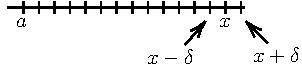
\includegraphics[scale=1]{T_Fcontinue.pdf}
                    \end{figure}
                    很容易想象,把$[a,x]$稍微变小$[a,x-\delta]$,那么根据连续性有:
            
                    于是这个时候根据变差的衔接性:
                    $$
                    T_F(a,x-\delta)\geq P+r_1
                    $$
                    $$
                    T_F(a,x)-\epsilon \leq P+r_1+\epsilon
                    $$
                    于是$T_F(x-\delta,x)<2\epsilon$。

                    现在考虑右边。我们只需要取一个比$x$大的数$b$。在$[x,b]$中的分划可以给出:
                    $$
                    \epsilon+P \geq L(B,C)-\epsilon,\qquad P\leq L(B_1,C)
                    $$
                    于是
                    $$
                    L(B,B_1)\leq 2\epsilon
                    $$
                    得证。
                \end{proof}
                \subsubsection{勒贝格引理}
                如果我们弄清楚了有界变差函数结构,那么一个自然的想法是,是否有界
                变差函数就是之前的牛莱公式的必要条件呢?(因为曲线可求长了)。我们想知道
                有界变差到底能多“符合”牛莱公式里面的条件。勒贝格先生给出了一个引理:
                \begin{theorem}
                    如果$F$是有限变差函数,那么$F$在$[a,b]$上几乎处处可导。
                \end{theorem}
                我们只用讨论单增的函数。在这之前,最好先讨论连续的情况,再来看一般情况。因为单调的函数
                不连续的点只有可数个。

                \begin{lemma}[日出引理]
                    假设$G$是一个实值函数,并且在$\R$上连续。假设$E$表示:
                    $$
                    \{x \in \R| \exists h=h_x>0,G(x+h)>G(x)\}
                    $$
                    那么$G$要么空,要么开集。如果是开集,
                    其可以写为:$\bigcup_{k=1}^\infty(a_k,b_k)$。此时,$G(b_k)-G(a_k)$。
                \end{lemma}
                证明我们略去。
                实际上,根据引理的名字——日出,
                可以用一座山和一个垂直上升的太阳来给出证明。

                严格的证明可以考虑二分法。
                \begin{corollary}
                    考虑$G(x)$在$[a,b]$连续。根据上述定理的证明,
                    $E=\bigcup_{k=1}^\infty (a_k,b_k)$。($E$是$(a,b)$子集)。
                    只有当$a_k=a$时我们允许$G(a_k)\leq G(b_k)$。其余时候都严格等于。

                \end{corollary}
                我们旋即给出勒贝格引理的证明:
                \begin{proof}
                    我们说明两件事:
                    $$
                    D^+(F)(x)=\limsup_{h \to 0^+}
                    \frac{F(x+h)-F(x)}{h}
                     <+\infty \qquad \text{for a.e. x}
                    $$
                    $$
                    D^+(F)(x)\leq D_{-}(F)(x) \qquad \text{for a.e. x}
                    $$
                    一旦这两件事成立,那么根据$-F(-x)$也是单增函数,我们就能有:
                    $$
                    D^{-}(F)(x)\leq D_{+}(F)(x) \qquad \text{for a.e. x}
                    $$
                    于是根据:
                    $$
                    D^+ \leq D_{-} \leq D^{-} \leq D_{+}\leq D^+\leq +\infty 
                    $$
                    知导函数几乎处处存在。

                    对于第一件事,我们说明
                    $$
                    E_\gamma=\{x: D^+ >\gamma\}
                    $$
                    的测度趋近于0($\gamma \to \infty$)。事实上,由于可测和极限作用下可测函数保持,所以$E_\gamma$
                    仍是可测集。我们让$G=F-\gamma x$,于是根据日出引理,由于$x \in E_\gamma$:
                    $$
                    E_\gamma \subset \bigcup_k (a_k,b_k)
                    $$
                    于是
                    $$
                    m(E_\gamma)\leq \sum_k (b_k-a_k)\leq \frac{1}{\gamma}\sum_k F(b_k)-F(a_k)=\frac{1}{\gamma}(F(b)-F(a))
                    $$

                    对于第二件事,我们可以用:
                    $$
                    \bigcup_{r,R\in \Q}\{x\in[a,b]:D^+ >R>r>D_{-}\}
                    $$
                    来表示$D^+>D_{-}$的集合。于是我们只用证上面的集合测度零。

                    假设$E=\{x\in[a,b]:D^+ >R>r>D_{-}\}$,
                    假设$m(E)>0$。那么存在开集$O:E\subset O$且$m(O)< R/r m(E)$。

                    取$O$区间分解中的$I_n$。在$-I_n$上对$G(x)=F(-x)+rx$
                    使用日出引理,于是有$\bigcup_k (a_k,b_k)\subset I_n$:
                    $$
                    F(b_k)-F(a_k)\leq r(b_k-a_k)
                    $$
                    此时对于$(a_k,b_k)$,$G(x)=F(x)-Rx$使用日出引理,于是有:
                    $$
                    F(b_{k,j})R(b_{k,j}-a_{k_j})
                    $$
                    此时$P=\bigcup_{k,j}(a_{k,j},b_{k,j})$满足:
                    $$
                    m(P)\leq \frac{1}{R}\sum_{k,j}{F(b_{k,j})-F(a_{k,j})}\leq 
                    \frac{1}{R}\sum_k F(b_k)-F(a_k)\leq \frac{r}{R}\sum_k (b_k-a_k)\leq \frac{r}{R}m(I_n)
                    $$
                    我们没有说明$P$不是空集。但是这可以由:
                    $$
                    P\supset I_n \cap E
                    $$
                    来得到。于是$m(E)=\sum_n m(E\cap I_n)\leq 
                    \sum_nr/Rm(I_n)=r/Rm(O)<m(E)$矛盾!

                    定理得证。

                \end{proof}
                冗长的证明其实非常宽松。在不等式的放缩中,
                我们给了许多宽泛的条件。
                比如$E_\gamma \subset \bigcup_k(a_k,b_k)$

                一旦有了勒贝格引理,我们就能给出下列结果:
                \begin{theorem}
                    如果$F$单调增,连续于$[a,b]$,那么$F'$几乎处处存在,并且$F'$可测非负,且:
                    $$
                    \int_a^b F'(x)dx \leq F(b)-F(a)
                    $$
                    特别的,如果$F$在$\R$有界,那么$F'$可积。
                \end{theorem}
                \begin{proof}
                    考虑可测函数$G_n(x)=\frac{F(x+1/n)-F(x)}{1/n}$这个函数的极限是$F'$。所以$F'$是可测的。于是我们可以
                    做形式的勒贝格积分:(Fatou引理)
                    $$
                    \int_a^b F'(x)dx \leq \liminf_{n \to \infty}\int_a^b G_n(x)dx
                    $$
                    展开$G_n$,有:
                    $$
                    \int_a^b G_n=\frac{1}{n}(
                        \int_b^{b+1/n}F(x)dx-\int_a^{a+1/n}F(x)dx)
                    $$
                    根据之前的积分的公式,我们得到:
                    $$
                    \int_a^b G_n \leq F(b)-F(a)
                    $$
                    于是得证。
                \end{proof}
                \begin{example}
                    等号是不能保证的。事实上,可以举出平凡的例子:只有做一个阶梯函数
                    就可以。显然$F(b)-F(a)>0$,但函数不连续。

                    我们指出,建立在Cantor集合上面的函数$F$是连续的,几乎处处导函数为0的函数。这给出了
                    连续情况下的反例。

                    具体情况看书即可。在第126页!
                \end{example}
                \subsubsection{绝对连续函数}
                到底要什么样的函数才能保证等号呢?这一节给出了答案——绝对连续函数。
                \begin{definition}
                    称$F$在$[a,b]$上绝对连续,如果对于任何$\epsilon>0$,都存在$\delta>0$使得:
                    只要$\sum_{k=1}^N(b_k-a_k)<\delta$,就有:
                    $$
                    \sum_{k=1}^N |F(b_k)-F(a_k)| \leq \epsilon
                    $$
                    其中$(a_k,b_k)$是不相交的。
                \end{definition}
                \begin{proposition}
                    \begin{enumerate}
                        \item 绝对连续函数一致连续。
                        \item 绝对连续函数有界变差。其变差函数当然也是连续的。
                        \item 积分函数$\int_a^x f(t)dt$在$f(t)$可积的时候绝对连续。
                    \end{enumerate}
                \end{proposition}
                    \begin{proof}
                        说明3.事实上,由于勒贝格积分在被积分区域测度足够小的时候,积分值
                        也足够小,那么立马就得到积分函数绝对连续。
                    \end{proof}
                命题3.3的第三条给出了曙光:
                \begin{theorem}
                    绝对连续函数$F(x)$在$[a,b]$上几乎处处可导。如果$F'(x)=0$几乎处处成立,那么
                    $F'(x)$是常数。
                \end{theorem}
                我们来分析一下证明。首先,如果$E$表示可导集,那么$m(E)=b-a$。如果在不可导的点,我们证明
                其发生的变化可以任意小即可。为此,我们先用一个性质来覆盖$E$.
                \begin{definition}
                    一个球族$\mathcal{B}$被称为是$E$的Vitali覆盖,如果对于
                    任意的$\eta>0,x \in E$,都有一个球$B \in \mathcal{B}$使得:$x \in B$,$m(B)\leq \eta$。
                \end{definition}
                \begin{lemma}[Vitali覆盖引理2]
                    假设$E$是一个有限测度的集合,$\mathcal{B}$是它的Vitali覆盖。那么对于
                    任意的$\delta>0$,都能找到有限多个不交的球$B_1,\dots,B_N$满足:
                    $$
                    \sum_{i=1}^N m(B_i)\geq m(E)-\delta
                    $$
                \end{lemma}
                \begin{proof}
                    不妨令$\delta <m(E)$。于是根据可测集测度被紧子集逼近的性质,我们可以找到
                    一个紧集$E_1$满足:$m(E_1)\geq \delta$。根据有限覆盖定理,有有限个球覆盖$E_1$。

                    从而有有限个不交的球$B_1,B_2,\dots,B_{N_1}$是之前有限个球的一部分,
                    且满足:
                    $$
                    \sum_{k=1}^{N_1} m(B_k)\geq 3^{-d} m(E_1)\geq 3^{-d} \delta
                    $$
                    
                    如果$3^{-d}\delta \geq m(E)-\delta$,那么我们证明结束。如果不能,考虑集合
                    $E_1=E-\bigcup_{k=1}^{N_1}$。注意到$m(E_1)\geq \delta$,并且根据
                    Vitali覆盖的性质,$E_1$仍被集族$\mathcal{B}$去除$B_1,\dots,B_{N_1}$
                    Vitali覆盖.于是同样的操作。

                    这样,有限次操作后,我们把找到的球全部合起来,就一定能在某一步时,让
                    $$
                    \sum_{k=1}^N m(B) \geq m(E)-\delta                    $$
                \end{proof}
                \begin{corollary}
                    可以安排$B_k$使得其满足:
                    $$
                    m(E-\bigcup_{i=1}^N B_i) <2\delta
                    $$
               \end{corollary}
               事实上,找一个开集把$E$包含住,$m(O-E)<\delta$。由于$O$是开集,于是$E$的Vitali覆盖
               可以全部限制在$O$里面。此时:
               $$
               m(E-\bigcup_{i=1}^N B_i)\leq m(O)-\sum_{i=1}^N m(B_i) \leq m(E)+\delta-(m(E)-\delta)=2\delta
               $$
               \begin{proof}[定理3.3.9]
                   现在我们给$E$找一个Vitali覆盖。一方面,选出来的区间要增长的比较慢。
                   另一方面,没有被选出来的空间要足够的小,使得根据绝对收敛,在这个区间上能变化的
                   值也很小。

                   对于第一方面,我们发现,对于任意的$x \in E$,由于导函数为零,所以能找到$(a_k,b_k)$满足:
                   $$
                   |F(b_k)-F(a_k)| \leq \epsilon(b_k-a_k), b_k-a_k <\eta
                   $$
                   这样就给出了$E$的Vitali覆盖.并且在这些不交区间(根据引理,我们已经选出来了)中,增长的速度很慢(小于$\epsilon$)。

                   同时,这些区间与$E$的测度差距小于$\delta$。根据绝对收敛,得到在这些区间上
                   总变差小于$\epsilon$。于是:
                   $$
                   |F(b)-F(a)| \leq \epsilon(b-a)+\epsilon
                   $$
                   $\epsilon$时任取的。(在研究导数时就取出了)。
               \end{proof}
               注意,证明中有三个小量。$\epsilon$描述了变化速度,$\eta$描述了覆盖的区间长度(即表明时Vitali覆盖),$\delta$表明了剩下不可导区间
               的长度,其正好能使$F$在上面的变差小于$\epsilon$。
                \begin{corollary}
                    假设$F$是$[a,b]$绝对连续的函数。那么就有:
                    $$
                    F(x)-F(a)=\int_a^x F'(y)dy
                    $$

                \end{corollary}
                \begin{proof}
                    考虑函数$G=\int_a^x F'(y)dy$。则$G'=F'$于是$G$与
                    $F$只相差常数,命题得证。
     
                    
                \end{proof}
                \subsubsection{跳跃函数}
                我们已经研究了连续函数的勒贝格引理。由此我们得出了牛莱公式取等号和小于号的一些条件。

                如果函数想要满足牛莱公式,绝对连续是一个充分条件。从而我们只讨论单调,不连续函数的导函数存在性问题。

                然而单调函数的不可导点是可数的,从而这些点实际上是很少的。通过分离,我们
                可以用一个连续函数和一个跳跃函数来描述单调函数。从而,我们想要研究“几乎处处可导”的话,
                只需要研究跳跃函数。
                \begin{definition}
                    一个函数被称为跳跃函数,如果其有如下的形式:
                    $$
                    f(x)=\sum_{k=1}^\infty a_k j_k(x)
                    $$
                    其中$j_k$是诸如:
                    \begin{equation*}
                        j_k(x)=\begin{cases}
                           1,\text{if }\quad x>x_k,\\
                           0,\text{if }\quad x<x_k.\\
                           \theta_k,\text{if}\quad  x=x_k.
                       \end{cases}
                       \end{equation*}
                       的函数。$0\leq \theta_k \leq 1$。
                \end{definition}
                容易看出,跳跃函数就是把一般的单调函数的不连续给抽了出来。抽出来后,还剩下一个单调的连续函数,这就符合我们
                于是我们想要研究单调函数,只用研究
                跳跃函数。
                \begin{theorem}
                    跳跃函数的导数几乎处处存在。从而单调函数的导数几乎处处存在,于是有界变差的的导数几乎处处存在。
                \end{theorem}
                \begin{proof}
                    这个定理并不是那么显然。我们不能在脑子里想一个阶梯函数。(也许会有一个点任何邻域
                    内都有跳的点)

                    给定任何$\epsilon>0$,我们证明集合$E$:
                    $$
                    \limsup_{h\to 0}\frac{J(x+h)-J(x)}{h}>\epsilon
                    $$
                    的测度是0.事实上,我们取:
                    $$
                    J_0(x)=\sum_{n>N}\alpha_n j_n(x)
                    $$
                    那么,只要$N$足够大,后面的函数就一致收敛到0.从而我们先考虑前面的$N-1$项。

                    并且$J_0(b)-J_0(a) <\eta$。$\eta$是任意给定的,与$N$相关。

                    前面的$N$项是有限的,从而显然,其不可导的点只有$x_1,x_2,\dots,x_N$。如果我们用$J_0$代替$J$,那么$E$中只会
                    减少有限个点。

                    设$E$的测度是$\delta$。那么$E$有紧子集$K$:$K\cap \{x_1,\dots,x_N\}=\emptyset
                    $,$m(K)>\delta/2$。对于$x \in K$,根据前面所说的,存在$(a_x,b_x)$
                    使得$x \in (a_x,b_x)$并且:
                    $$
                    J_0(b_x) -J(a_x) >\epsilon(b_x-a_x)
                    $$
                    这里我们替换上$J_0$。因为$(a_k,b_k)$只要小一些,
                    就能避开$x_1,\dots,x_N$,从而前$N$项一样。

                    于是根据有限覆盖,得到:
                    $$
                    \sum_{j=1}^n m(I_j) \geq m(K)/3
                    $$
                    于是$J_0(b)-J_0(a)\geq \sum_{j=1}^N J_0(b_j)-J_0(a_j) \geq \epsilon\sum
                    (b_j-a_j) >\epsilon/6 \delta$

                    于是$\eta>\epsilon \delta/6$。根据$\eta$任意性,得证。
                \end{proof}
                这几个定理的证明都用到了Vitali覆盖引理。其引理在于,只要某种
                性质的开集能够覆盖一个集合,那么就能从集族中扣出来一些不相交的集合,使得这些不相交
                的集合与原来被覆盖的集合测度,差距相当小;于是在这个测度足够小的地方,我们能
                做很多事情(比如绝对连续能干什么之类的。)。同时,在这些不相交的集合上,我们能做放缩。由于几乎就是原覆盖集合
                从而我们能保证这些放缩最终影响被覆盖的集合。
                \subsection{Minkowsky内含与等周不等式}
                在研究了对导函数积分的问题后,我们转而对曲线的可求长性进行更加深入的研究。我们想要验证下列公式
                的正确性,或者成立的条件:
                $$
                L=\int_a^b |z'(t)|dt
                $$
                其中我们的曲线为:$z(t)=x(t)+iy(t),a\leq t\leq b$。

                显然这个式子是不一定成立的。只用令$x(t)=F(t)=y(t)$,$F(t)$是康托-勒贝格函数。从而
                $F'(t)=0$,于是积分为零。但是整根曲线的长度是$\sqrt{2}$。矛盾!

                不难想到,如果是绝对连续的,那么公式就成立了:
                \begin{theorem}
                    $$
                    L=\int_a^b |z'(t)|dt
                    $$
                    在$G(t)=z(t)$绝对连续的时候成立。
                \end{theorem}
                定理的证明,我们将给出一个命题。这个命题说明了上述定理的
                成立。
                \begin{proposition}
                    设$F$是复值绝对连续函数,定义域$[a,b]$。那么:
                    $$
                    T_F(a,b)=\int_a^b |F'(t)|dt
                    $$
                \end{proposition}
                \begin{proof}
                    我们先证明小于等于,再证明大于等于。
                    
                    $\leq$:给出$a=t_0 <t_1<t_2<\dots<t_N=b$。于是:
                    $$
                    \sum_{k=1}^N |F(t_{k})-F(t_{k-1})|=\sum_{j=1}^N|\int_{t_{k-1}}^{t_k}F'(t)dt|\leq \sum_{k=1}^N\int_{t_{k-1}}^{t_k}|F'(t)|dt =\int_a^b|F'(t)|dt
                    $$
                    于是取上确界就得到结果。

                    $\geq$:我们思考,什么样的函数会显而易见的满足上述等式?如果$F'(t)=0$就可能。而$F'(t)=0$代表了
                    步函数。步函数和一般的函数是足够的接近的。

                    固定$\epsilon>0$,存在$g$在$[a,b]$
                    使得:$F'=g+h$,$\int_a^b|F'-g|dt=\int_a^b|h|dt\leq \epsilon$.
                    定义$G,H$是对应的积分函数,从而$F=G+H$.

                    考虑$|G|\leq |F-H| \leq |F|+|H|$:
                    $$
                    T_F(a,b) \geq T_G(a,b)-T_H(a,b)
                    $$
                    由于$T_H(a,b)\leq \int_a^b |h|dt <\epsilon$:
                    $$
                    T_F(a,b)\geq T_G(a,b)-\epsilon
                    $$
                    只要说明$T_G(a,b)$等于$\int_a^b |g|dt$,并且$\int_a^b |g|dt$与$F$的差不多就可以。
                    这是明显的。于是:
                    $$
                    T_F(a,b)\geq \int_a^b|F'(t)|dt-2\epsilon
                    $$
                    证毕。
                \end{proof}
                从理论上,我们可以对任何可求长的曲线给出“自然参数”。这只有理论的意义,但有助于我们把问题
                变为积分来考量。

                记$s(t)=L(a,t)$。即$s(a)=0,s(b)=L$。由于我们假定参数都是连续的,因此$s$是连续单增的。

                做变量替换,于是$z(t)=\tilde{z}(s)$.这个替换是良定的。因为如果$t_1<t_2$,$s(t_1)<s(t_2)$,
                那么$z(t_1)=z(t_2)$。这不是我们所能容许的。

                这样的替换保证了$|\tilde{z}(s_1)-\tilde{z}(s_2)| \leq |s_1-s_2|$.因此绝对连续满足。于是
                $$
                L=\int_0^L |\tilde{z}'(s)|ds
                $$
                \subsubsection{Minkowski内含}
                \begin{definition}
                    曲线$z(t)=x(t)+iy(t),a \leq t\leq b$被称为拟简单曲线,若映射$z \mapsto z(t)$除了$[a,b]$中的有限个点都是单射。
                \end{definition}
                用$\Gamma$表示$\{z(t):a \leq t\leq b\}$。根据连续性,这是一个
                紧集。从而我们用$K^\delta$表示:
                $$
                K^\delta=\{x \in \R^2:d(x,K)<\delta\}
                $$
                其中$K$是任意一个紧集。把$\Gamma$记为$K$,我们定义:
                \begin{definition}
                    紧集$K$有\textbf{Minkowski内含},如果:
                    $$
                    \lim_{\delta \to 0}\frac{m(K^\delta)}{2\delta}
                    $$
                    存在,记为$\mathcal{M}(K)$.
                \end{definition}
                \begin{theorem}
                    设$\Gamma$是一个拟简单曲线。$\Gamma$的Minkowski内含存在,当且仅当其可求长。并且
                    当上述条件满足时,$\mathcal{M}(\Gamma)=L$.
                \end{theorem}
                为了证明定理,我们考虑下列两个量:
                $$
                \mathcal{M}^*(K)=\limsup_{\delta\to 0}\frac{m(K^\delta)}{2\delta}
                $$
                $$
                \mathcal{M}_*(K)=\liminf_{\delta\to 0}\frac{m(K^\delta)}{2\delta}
                $$
                \begin{proposition}
                    如果$\mathcal{M}_*(\Gamma)<\infty$,那么曲线可求长,并且:
                    $$
                    L \leq M_*(\Gamma)
                    $$
                \end{proposition}
                证明该命题需要一个简单的观察:
                \begin{lemma}
                    $$
                    m(\Gamma^\delta)\geq 2\delta |z(b)-z(a)|
                    $$
                \end{lemma}
                \begin{proof}
                    通过把$z(a),z(b)$移动到$x$轴上,我们可以考虑
                    下面这个图:
                    \begin{figure}[htbp]
                        \centering
                        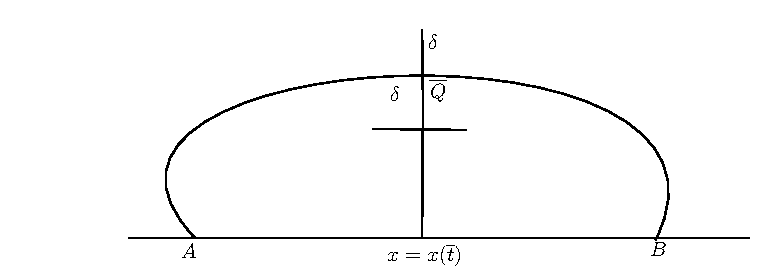
\includegraphics[scale=0.6]{delta.pdf}
                    \end{figure}

                    利用Fubini定理,积分换序就能得到答案。
                \end{proof}
                \begin{proof}
                    引理启发我们,
                如果我们把整个曲线分为若干段,
                再把每段做的略略缩小,
                那么既可以达到两点:
                
                1.每个段的$K^\delta$不相交。

                2.每个段的和与整个折线长度相差很小。

                从而就能证明定理。我们只说明了简单曲线的情况。拟简单曲线的情况是类似的。只要把
                不是单调的那些点,连同周围的一个小区域给扣掉即可。
                \end{proof}
                
                
            \end{document}
